
\ifx\isEmbedded\undefined

\pdfobjcompresslevel 0
\documentclass[a4paper, 12pt]{report}


%
%%\usepackage{comment} % Permet de compiler sans les figures et sans les tables
%%\excludecomment{figure}
%%\let\endfigure\relax
%%\excludecomment{table}
%%\let\endtable\relax

%\usepackage{refcheck} %permet de voir les refs du bib non cit�es

\setlength{\parindent}{0pt} %get rid of indentation in the article
\usepackage{etoolbox} % prevent a Patching '\begin' failed! see https://tex.stackexchange.com/questions/128938/package-etoolbox-warning-patching-begin-failed
%\usepackage{natbib} % pour bibtex \citep (parenthetical) et \citet (textual) (sinon seul \cite marche) a loader avant babel
\usepackage[semicolon,round,sort&compress,sectionbib]{natbib}  %
\usepackage{chapterbib}      
\usepackage[english, french]{babel} %Fran�ais à loader avant caption
\usepackage[T1]{fontenc}

  \usepackage{adjustbox}
\usepackage[affil-it]{authblk} %for affiliation
\usepackage{afterpage} % To include blanck page with command \afterpage{\blankpage}
\usepackage{appendix}

\usepackage{array} %pour les tableaux
\usepackage{amsmath, amssymb} %american mathematical society math style and symbols (amssymb)
\usepackage{amsthm}
\usepackage{blindtext}
\usepackage{booktabs}
\usepackage{breqn} % allow to use dmath environment (automatic break for equations, etc) 
\usepackage{caption} % Needed to jump line in figures titles (caption).
%\usepackage{commath} sais pas pourquoi �a marche pas si je charge �a plante !

\usepackage{dirtytalk} % quote stuff with \say{the text to quote}
\usepackage{empheq} %
\usepackage[official]{eurosym}  %type \euro{} to print a euro
\usepackage{float} % for firgure placement with H option
\usepackage{fancybox}

  \usepackage[top=2cm, bottom=2cm, left=2.5cm, right=2.5cm]{geometry}
  \usepackage[top=2cm, bottom=2cm, left=2.5cm, right=2.5cm]{geometry}
\usepackage{graphicx} %pour ins�rer des images.
 \usepackage[hyperindex=true,
 		     colorlinks=true, 
		     urlcolor=blue,
		     citecolor    = blue, %Couleur des citations (biblio)
    		     linkcolor    = blue, %Couleur des équations. Apparemment, cela sert aussi pour théoreme, Lemme...
 					 ]{hyperref} %permet de mettre des hyper liens (le package url le fait tout seul ? la base)

\usepackage{import}					 



\usepackage{pdflscape}
\usepackage{pdfpages} %allow to select which pdf pages to compile 
\includepdf[pages={12-15,23,45-49}]{main.pdf} 
\usepackage{spverbatim}
\usepackage{lmodern}%change un peu les lettres pour un truc plus cool, marche peut �tre un peu mieux avec les accents v�rifier � l'occaz
\usepackage{mathrsfs} % allows $\mathscr{ABC}$ to work
\usepackage{setspace} % permet de d�terminer une largeur d'interligne
\usepackage{tikz} % draw graphs
\usetikzlibrary{trees,shapes,snakes}
  \usepackage{subcaption} % to use with subfigures
\usepackage{skull}
\usepackage{url}
\usepackage{verbatim} %Pour ins�rer du code informatique

\usepackage{fancyvrb}
\usepackage{fvextra}

\usepackage{array} %one of the two needed to use thead to break line in tabular
\usepackage{makecell} %one of the two needed to use thead to break line in tabular

\DeclareUnicodeCharacter{20AC}{\euro{}}
\DeclareUnicodeCharacter{2212}{-}
\DeclareUnicodeCharacter{300}{`}
\DeclareUnicodeCharacter{301}{'}

  \newcommand{\hdrule}{\midrule[\heavyrulewidth]}

\newsavebox{\mybox}

\newcommand{\raisedshadowbox}[1]{%
\sbox\mybox{\shadowbox{#1}}%
\raisebox{-0.5\ht\mybox-0.5\shadowsize+0.6ex}{\usebox\mybox}%
}
%%%%%
\providecommand{\tightlist}{%
  \setlength{\itemsep}{0pt}\setlength{\parskip}{0pt}}


\bibliographystyle{chicagoa}


%%%%%%%%%%%%%%%%
%%%Fin biblio %%%%%%%%



%%%%Elispse in tables%%%%%%
\usepackage{tikz}
\usetikzlibrary{fit,shapes.misc}
\newcommand\marktopleft[1]{%
    \tikz[overlay,remember picture] 
        \node (marker-#1-a) at (0,-1ex) {};%
}
\newcommand\markElipseBottomright[1]{%
    \tikz[overlay,remember picture] 
        \node (marker-#1-b) at (0.2,0.3) {};%
    \tikz[overlay,remember picture,thick,dashed,inner sep=3pt]
        \node[draw, ellipse,fit=(marker-#1-a.center) (marker-#1-b.center)] {};%
}
%%%%End Elispse in tables%%%%%%






%%%%Squares in tables%%%%%%
\newcommand\markRectangletopleft[1]{%
    \tikz[overlay,remember picture] 
        \node (marker-#1-a) at (0,1.5ex) {};%
}
\newcommand\markRectanglebottomright[1]{%
    \tikz[overlay,remember picture] 
        \node (marker-#1-b) at (0,0) {};%
    \tikz[overlay,remember picture,thick,dashed,inner sep=3pt]
        \node[draw,rounded rectangle,fit=(marker-#1-a.center) (marker-#1-b.center)] {};%
}
%%%%Squares Circles in tables%%%%%%


\newcommand\blankpage{%
    \null
    \thispagestyle{empty}%
    \addtocounter{page}{-1}%
    \newpage}




\DeclareMathOperator\erf{erf}


\providecommand{\U}[1]{\protect\rule{.1in}{.1in}}
%EndMSIPreambleData
\newtheorem{theorem}{Theorem}
\newtheorem{acknowledgement}[theorem]{Acknowledgement}
\newtheorem{algorithm}[theorem]{Algorithm}
\newtheorem{axiom}[theorem]{Axiom}
\newtheorem{case}[theorem]{Case}
\newtheorem{claim}[theorem]{Claim}
\newtheorem{conclusion}[theorem]{Conclusion}
%\newtheorem{condition}[theorem]{Condition}
\newtheorem{conjecture}[theorem]{Conjecture}
\newtheorem{corollary}[theorem]{Corollary}
\newtheorem{criterion}[theorem]{Criterion}
\newtheorem{definition}[theorem]{Definition}
\newtheorem{example}[theorem]{Example}
\newtheorem{exercise}[theorem]{Exercise}
\newtheorem{lemma}[theorem]{Lemma}
\newtheorem{notation}[theorem]{Notation}
\newtheorem{problem}[theorem]{Problem}
\newtheorem{proposition}[theorem]{Proposition}
\newtheorem{remark}[theorem]{Remark}
\newtheorem{solution}[theorem]{Solution}
\newtheorem{summary}[theorem]{Summary}
%\newenvironment{proof}[1][Proof]{\noindent\textbf{#1.} }{\ \rule{0.5em}{0.5em}}



\usepackage{fancyhdr}

\usepackage{minitoc} % table of contents should be loaded after hyperef and other packages
\usepackage{silence}


%%%%% Mute minitoc warnings see https://tex.stackexchange.com/questions/166910/what-are-these-warnings-for-minitoc-package
\WarningFilter{minitoc(hints)}{W0023}
\WarningFilter{minitoc(hints)}{W0024}
\WarningFilter{minitoc(hints)}{W0028}
\WarningFilter{minitoc(hints)}{W0030}
\WarningFilter{blindtext}{} % this takes care of the `blindtext` messages

\usepackage{grffile}

\graphicspath{{}}

\frenchbsetup{ShowOptions} 

\Urlmuskip=0mu  plus 10mu  %Solver Overfull \hbox for url links (see https://tex.stackexchange.com/questions/339682/how-to-really-solve-the-problem-of-underfull-hbox-when-typesetting-url-in-f)
\graphicspath{{figures/}}
\begin{document}
\setcounter{chapter}{6}
\chapter{\label{??} ??}
\else \fi

%%%%%%%%%%%%%%%%%%%%%%%%%%%%%%%%%%%%%%%%%%%%%%%%%%%%%%%%%%%%%%%%%%%%%%%%%%%%%%%%%%%%%%%%%%%%%%%%%%%%%%%%%%%%%%
\setstretch{1.5}
\noindent 

The pioneering work of Vickrey (1939, 1947) on the income-tax
frequency has not inspired a lot of further studies. We propose an
investigation of this issue both from a theoretical and empirical viewpoint
within the year. We first show that increasing the income-tax frequency (from
an annual tax basis to a monthly tax basis) and refunding the extra-revenue
for the taxpayer is Pareto-improving for any convex tax scheme (increasing
marginal tax) and any risk-adverter. Welfare gains are all the larger as the
infra-annual volatility of income is large and the possibility to borrow is
low, implying that the benefits should be larger for the bottom part of the
income distribution. We submit an empirical illustration using French
administrative tax data and simulations of the current tax-benefit system.
Despite that this system is not convex over the whole income domain, we show
that increasing the tax frequency can lead to substantial social welfare gains. 
However the average welfare gain is lower with the proposed system than with the Vickrey's one even though there are less losers.



\newpage
\section{Introduction}

Time and risk are difficult matters and the design of tax system does not make
an exception when it deals with incomes which are not steady. Usually, the
practionners are applying some methods which are both understandable by the
layman and easy to implement. For instance, in withholding income tax systems,
tax collection is based on monthly income while tax schedules are designed
over yearly income, and filing at the end of the year allows using tax
allowances to obtain rebates. Benefits also have specific timing of income
assessment (for instance in France, earnings of the three past months form the
basis of means-tests for social assistance and in-work benefits). Effective
taxation then possibly treats various time periods and, hence, different
streams of income differently. In this paper, we question the welfare
implications of varying the period of observation of the tax base within a year.

Arguably, our question would be irrelevant if people had constant income flows
over time. Yet it is clear that many households do face important income
variation during the year, either expected (pay rise, seasonal work) or
unexpected (income shocks due to business failure or unemployment), voluntary
(chosen retirement) or involuntary (low-skill workers forced into temporary
work). This is a major motivation for studying the question of within-year tax
frequency and its impact on tax-payer utility. Note also that our question
would be meaningless if effective taxation was flat. However, this never
happens. Effective taxation, i.e. the impact of taxes and benefits, is usually
nonlinear. Even in flat-tax countries, the presence of many other instruments,
e.g. means-tested benefits, impose some regressivity or progressivity upon the
effective tax schedule.

Interestingly, and potentially important for our welfare analysis, the
question of tax frequency may be more relevant at the bottom of the
distribution. Indeed, for high income households, large income variations are
usually required to change tax brackets (especially given the global trend
that has consisted in reducing the number of brackets, \citet [Fig. 3,
p.468]{sabirianova_reform_of_pit}). For them, this is as if they faced a
marginal flat tax around the pre-shock income level. In the lower part of the
distribution, however, effective brackets are narrower because of the numerous
(and often overlapping) redistributive schemes at low and middle income levels
(e.g. social assistance, tax credits, means-tested family benefits, etc.).
Thus, even small variations of income may lead to change in effective marginal
tax rates (MTR). There is also empirical evidence that this population
experience more income fluctuations, and that income variation is more often
involuntary, e.g. income shocks due to unemployment \citep{Hills2006}. These
aspects are likely to contribute much to the welfare implications of tax
frequency that we shall study.\footnote{Note also that poorer people are less
able to smooth income because lower resources limit their saving possibilities
(\citet {dynan2004rich} finds a median saving rate of 1 percent for households
in the bottom quintile for US households aged 30-59). In addition, they are
often more credit constrained and possibly more myopic (cf. Hastings and
Washington, 2010).}\bigskip

Strangely enough, the question of tax temporality has received little
attention in the economic literature. Very few studies make the link between
tax-payer utility and tax temporality. The seminal work of \citet
{vickrey1939averaging} focuses on yearly versus lifetime taxation. Vickrey
develops the horizontal equity argument that over the lifecycle, people
earning the same income should pay the same tax. This leads William Vickrey to
propose the celebrated "Cumulative Averaging" tax principle.\ Initially, the
idea was formulated for taxing capital gains and then extended to other types
of income. The idea was that an investor should have no incentive to realize
her capital gain at one time rather than another on account of the tax. The
upshot is that the tax should be completly neutral with respect to the time at
which the gain is realized\footnote{Vickrey's contribution has triggered
important advances in capital taxation (Auerbach, CITE) and dynamic optimal
taxation (CITE). An interesting extension of Vickrey's setting is
\citet {liebman2002should}. He studies a distributionally-neutral Vickrey tax
system that would equalize MTRs both over-time for the same individual and
across individuals with the same lifetime earnings level, incorporating
various motives for efficiency and equity gains (income shocks, myopic
agents). Finally, note that the temporality of taxation has also received some
attention in law studies following Vickrey, for instance
\citet {batchelder2003taxing} and \citet
{fennell2005taxation}.}.\ 

The present research is devoted to the temporality of the tax within a
year.\ Most developed countries operate a wage withholding tax
system\footnote{For capital incomes and earnings of self-employed, the tax
payment usually remains on a yearly basis.} which represents the benchmark
system in our reasoning. As already mentioned, the amount withheld and paid by
the employer to the government each month is applied as a prepayment of income
taxes and is refundable if it exceeds the income tax liability. The tax
liability is determined by filing the tax return at the end of the year and
applying the tax schedule including tax deductions. The current system is far
remote from applying a cumulative averaging system \`{a} la Vickrey.\ The
first idea which comes out is then to apply the cumulative average proposition.\ 

Three ingredients are needed to compute the tax liabilities according to the
cumulative averaging formula: a starting date, a termination date and a tax
schedule appropriate to the period covered.\ The idea of a termination date
raises some difficulty for applying the principle over the life cycle because
the time of death is uncertain.\ This difficulty vanishes when applying the
mechanism within a year. Each month the taxpayer is paying a withhold
tax.\ This tax is computed as the difference between the theoretical tax
liability of the subperiod running until that month minus the cumulated
withheld taxes of all previous months.\ Two mathematical operations are
performed to compute the former.\ First, the taxbase is computed on a annual
basis by assuming that the monthly average income since the beginning of the
year will prevail until the end of year.\ Second, the tax liability is
computed on a pro rata temporis basis.\ That is, the theoretical tax liability
for the five first months in May is only the 5/12 of the annual tax liability.

The extension of Vickrey's idea on earnings is not without dispute.\ Two
arguments can be stressed.\ From a more philosophical view point, we can
remind Derek Parfit's provocative stance: \textit{The difference between
different persons at the same time is more like the difference between the
same person at different times}. That difference in income over time should be
taken as a difference in ability to contribute over each period of time. A
sport superstar who is able to earn a lot of money over a period of 10 years
is a different man from what he will become years after. It is very in line
with the static Mirrlees optimal tax model with the efficiency equity
tradeoff. Vickrey's tax scheme looks at equity over the life cycle, but if
Derek Parfit view is embodied, equity is sacrified for efficiency.

Second it can be emphasized that in many ways human capital is different from
financial capital. If the capital market is liquid, you can sell your asset
when you want. The labor market is less liquid at least in a given year than
the capital market.\ In many places and many times, for different reasons that
we do not develop, the wage does not clear. It means that from the view point
of an individual the variability of earnings within a year reflect not only
preferences but also features on the local labor market demand as
aforementioned. We name the latter the unvoluntary variability. In that case,
neutrality with respect to time is not the only property we may want to see
respected by the income tax payment. Because of risk aversion, tax smoothing
is arguably a property that will come high on the list.\ The cumulative
averaging tax schedule is smoothing the payment of the tax within a
year.\ However it is not the only one and we are here investigating other mechanisms.\ 

In particular, there is a main difference between the framework that we deal
with and Vickrey's one.\ The big strength of the cumulative average formula is
each month payment to only depend on the available information.\ Each month,
there is a kind of bayesian revision of what the taxpayer owes, by
incorporating the earning information that is disclosed that month. We here
adopt a perfect information framework for tax authorities.\ Namely, the tax
authority knows the within-year income stream of the taxpayer from the
beginning of the year. This is of course unrealistic, even if there are
(econometric) means for the tax authority to forecast the variability of
income that prevails for different types of taxpayer.\ We will comment on that
in the conclusion.\ However we claim that at least from a theoretical
perspective and maybe more than that, it is always interesting to compare what
we could do in a context of perfect information and what we can do in a
context of available information.\ The difference represents the cost of uncertainty.\ 

In contrast, instead of averaging the income basis of each month, we consider
the opposite direction which is to increase the frequency of the tax within
the year,empirically illustrated with a move from annual to monthly taxation.
The tax liability will be monthly based. If the tax scheme is convex
(marginally progressive), the taxpayer will pay more with a monthly tax
liability than with an annual tax liability. We show that it is possible to
refund each taxpayer the extra amount of taxes and any risk-adverter tax payer
will be happier with this system termed the \textit{Monthly tax frequency with
compensation, }in short, \textit{Monthly compensated}. We should immediatly
stress that our proposal remains neutral with respect to the timing of income
within the year. Besides neutrality, there is the issue of welfare gains which
depend on the convexity of the tax schedule and the concavity of the utility
function, two features that are absent from Vickrey's paradigm.\ We are more
specific but we do not deviate from usual assumptions considered in economic theory.\ 

To the best of our knowledge, we are the first to study the welfare impact of
tax frequency within the year, in particular the implications of a shift from
annual to monthly taxation. We first suggest a simple theoretical framework in
which Jensen's inequality implies that a taxpayer with irregular income
streams will pay more with a monthly tax scheme. We derive compensation
schemes for the increase in tax liability due to income variation, i.e.
compensations equating the amount of tax paid in both annual and monthly
systems. We show that the reform with compensation is Pareto improving if
utility is increasing, concave and intertemporally additive. \footnote{At the
center of our theoretical results, \citet {varian1980redistributive}
emphasizes the insurance property of an income tax and shows in a two-period
model that this insurance component leads to a convex optimal tax scheme.} We
characterize those most concerned by welfare gains, namely those whose incomes
vary much over time and who face borrowing constraints.

We then submit an empirical illustration using French administrative data (tax
filing data combined with work sequences from the French Labor Force surveys
(\textit{Enqu\^{e}te Revenus Fiscaux et sociaux ERFS}). Using simulations of
the current income tax, we implement the higher-frequency tax reform and
characterize winners and losers. We extend this empirical exercise to
effective taxation, i.e. we additionally account for the main redistributive
scheme in France. While our Pareto improving results require the income tax to
be convex, real-world effective taxation is rarely so. Moreover, non-convex
parts of the effective schedule are typically located in the first half of the
income distribution, with the cumulative effect of different instruments (tax
credit and benefit withdrawals, social contributions and income tax, etc).
Despite this feature, which is particularly present in the case of French
taxation, we show that increased tax frequency with compensation leads to
substantial welfare gains.

The article is organized as follows. Section 2 presents our theoretical
framework and results. Section 3 shows descriptive statistics on France
taxpayers earnings. Section 4 submits simulation of a tax frequency reform on
French data while section 5 concludes.

\section{Theory}

The assessment of the tax determines the amount an individual is entitled to
pay based on its situation (income streams, family situation, etc). The
determined amount known as tax liability leads to a payment of the tax either
directly by the taxpayer, or by a third party institution (employer, banks,
etc). Appart from the frequency of the assessment of the tax, it can leads to
different schedule of payments. In practice in countries with Pay-as-you-earn
(PAYE) systems, an amount is withholded at each payroll period which can be
viewed as sub-periods of taxation, even though in most countries final tax
liability is computed over whole year incomes. Meaning that tax liability is
based on yearly income, but tax payments are made before the full realisation
of incomes that constitutes the tax base.

Hence, there exists a \emph{reference period} for the tax base in order to
determine th teax liability. In cases the government wish to recover taxes
before full realisation of income, it may want to apply some rules on
sub-periods to compute \emph{sub-period tax liability} based on income,
concomitant with the curent sub-period, or based on past income streams.

Those cumulative payments may lead to some differences with respect to tax
liability and may imply some implicit lending or borrowing between the
taxpayer and the state: in the US, fiscal household has to fill a tax return
in April for last year income to pay (or get refunded) the difference between
the withholded amount and the tax liability. France is moving slowly to a
withholding system which is due to be implemented in 2019.

We first define the framework, then expose five tax frequency regimes before
presenting some theoretical results about the comparison of the well-beings
they generate. We end the section by discussing the external validity of the
results when we embody behavioral reactions.

\subsection{Framework}

Let us consider a reference period $T$ and sub-periods $t$ from $1$ to $T$. If
we take the year length as the reference period and months as the single
periods, then T=12, and each month is labeled from 1 to 12. There are twelve
sub-periods corresponding to the first month, the two first months, the first
quarter and so on.\ We denote $y_{t}$ the gross income the taxpayer at period
$t=1,...,T$ with $y_{t}\geq0$. We call $G(.)$ the reference tax schedule, that
is the tax schedule for the reference period which is supposed to be
increasing and convex.\ $G$ can be positive (taxes) or negative (benefits). We
first study the case of positive taxes and then indicates how the analysis can
be extended to the case of a negative income tax. $z_{t}$ is the disposable
income or the net-of-tax income.

We define $G_{t}$ the \textit{pro rata temporis} single period tax schedule,
or in short, the sub-period equivalent tax schedule where $G_{t}=\frac{1}%
{T}G(Ty_{t}).$ The tax liability of period $t$ is denoted $g_{t}$.

In our proposal, sub-period equivalent tax function only depends of the
sub-period income. We should note that for equal income at each sub-periods
the reference income tax is just equal to the sum of the sub-period income
tax, formally :%

\begin{equation}
\sum_{1}^{T}\frac{1}{T}G(Ty)=G(\sum_{1}^{T}y),\forall y\in{{\mathbb{R}}}%
^{+}\label{non_varying_eq}%
\end{equation}


We consider that tax-payers have additive/separable utility functions defined
on disposable income:%

\begin{equation}
U=\sum_{t=1}^{T}u(z_{t})\,,\label{additive_u}%
\end{equation}


where $U$ is the reference period global utility function and $u_{t}$ is the
increasing and concave sub-period utility function of disposable income.
$u(.)$ can be viewed as the indirect utility function at constant wage and price.

At this stage, we do not include time discounting or interest rate in this
framework. These extensions are discussed in the discussion subsection as well
as behavioral responses to the change in taxation frequency.\ 

We recall the well-known mathematical result about partial sums and dominance
for a convex or concave function which will be useful in deriving results.

\begin{theorem}
Let $x$ and $y$ two income streams $x=(x_{1},...,x_{n})$ and $y=(y_{1}%
,...,y_{n})$, ranked in decreasing order, i.e., $x_{1}\geq x_{2}\geq\cdots\geq
x_{n}$ and $y_{1}\geq y_{2}\geq\cdots\geq y_{n}$ such that $\sum_{i=1}%
^{n}x_{i}=\sum_{i=1}^{n}y_{i}$ and $\sum_{i=1}^{k}x_{i}\geq\sum_{i=1}^{k}%
y_{i}$ for $k=1,...n-1.$ Then $\sum_{i=1}^{n}f(x_{t})\geq\sum_{i=1}^{n}%
f(y_{t})$ for any $f$ convex function.
\end{theorem}

The version of the theorem for a concave function holds for $x$ and $y$ two
income streams ranked in increasing orders. The obtained ranking of income
distributions corresponds then to the Lorenz ranking of income distributions.

\subsection{Five within-year tax payments}

\paragraph{Current payment}

In the US
\footnote{\url{https://www.irs.gov/publications/p505/index.html}\newline%
\url{https://www.irs.gov/pub/irs-pdf/p505.pdf}
\par
In fact, the adjustement is made in April after the taxpayer has filled his
tax return.} and in many countries, income tax is withholded by the employer
based solely on monthly income and monthly situation (family structure). At
the end of the year a tax adjustment is proceeded to make the total annual tax
liability exactly given by the reference period tax schedule.%

\[
g_{t}^{C}=%
\begin{cases}
\frac{G(Ty_{t})}{T}, & \mbox{if }t\in\lbrack1,11]\\
G(\sum_{1}^{12}y_{t})-\sum_{1}^{11}\frac{G(Ty_{t})}{T}, & \mbox{if }x=12.
\end{cases}
\]


\paragraph{Cumulated Averaging Tax}

Vickrey's proposal was that each sub-period payment should be equal to the
amount one would have paid under the sub-period tax schedule if the total
income had been earned in equal amounts in each single period composing the
sub-period. Without interest rate it leads to:
\begin{equation}
{g_{t}^{V}}=\frac{t}{T}G\left(  T\frac{\sum_{p=0}^{t}y_{p}}{t}\right)
-\sum_{p=0}^{t-1}{g_{p}^{V}}\label{eq:vickrey}%
\end{equation}
Where $g_{t}^{V}$ is the tax paid for a given single period $t$ with Vickrey's
tax scheme. On a year span, the taxpayer will have paid exactly the same
amount as in the current system $G(\sum_{1}^{12}y_{t})$. We can thus implement
a Vickrey's tax scheme on a yearly span -- instead of a lifetime span. This is
indeed the solutions that seems to be chosen by the Irish PAYE
system.\footnote{\url{http://www.revenue.ie/en/business/paye/guide/employers-guide-paye-calculation.html}}%


\paragraph{Equal Payment Regime}

In this system, the amount of the tax is based over income of the reference
period, $G(\sum_{1}^{T}y_{t})$. The tax is split equally between all the
single periods. If we denote $g_{t}^{E}$ the equal monthly payment made at
period $t$, then :%

\[
g_{t}^{E}=\frac{G(\sum_{1}^{T}y_{t})}{T}
\]


As a matter of fact, the Equal Payment Tax is not implementable since the
government has to know future income before their realisation. It can still be
used as a benchmark. Another limitation is that the monthly income should be
higher than the average tax liability, a constraint that can be viewed as severe.

\paragraph{Monthly Tax}

The monthly tax is the current tax without adjustment at the end of the year
\[
g_{t}^{M}=\frac{G(Ty_{t})}{T}.
\]


With a strictly convex tax function those with varying income will pay more
tax over the reference period with the montly tax than with the tax on the
reference period.%
\[
\sum_{1}^{T}\frac{G(Ty_{t})}{T}\geq G(\sum_{1}^{T}y_{t}))
\]


Concerning the utility of the tax-payer, its single period utility might be
lower or higher with the monthly tax than with the equal payment tax. Two
opposite effects are in play: the first one is that more tax is paid with the
sub-period tax, which reduces overall income, and thus overall utility. But on
the other hand, the fact that the tax is directly linked to the single period
income is smoothing the disposable income with a convex tax scheme. The
taxpayer pays a smaller tax when earning little and a bigger tax when earning
a lot. A risk adverter will like the reduced risk. On the whole, the effect is
ambiguous with a mean loss and a reduced variance. The effect depends thus on
the shapes of the tax and of the utility function, but also on the different
income streams and their dispersion around the annual mean.

\paragraph{Monthly Compensated Tax}

It is easy to equalize total tax assessement between the equal payment tax and
the sub-period tax. We just need to define the parameter $\lambda$ which will
decrease the single period tax schedule and wipe out the extra-tax collected
with a monthly taxation scheme.
\begin{equation}
\sum_{1}^{T}\frac{1}{T+\lambda}G(Ty_{t})=G\left(  \sum_{1}^{T}y_{t}\right)
.\label{compensation_eq}%
\end{equation}


$\lambda$ is a function of both the convexity of the tax function and the
variability of income over the year.\ It is positive or null.\
\[
\lambda(y,G)=\frac{\sum_{1}^{T}G(Ty_{t})}{G\left(  \sum_{1}^{T}y_{t}\right)
}-T.
\]


The uncertainty about the income stream should be resolved to compute the
parameter $\lambda$. Observe also that the value of $\lambda$ is specific to
the income realization of a given taxpayer. We will come back to that point on
the discussion sub-section. The tax paid for the monthly compensated tax (MC)
is then:
\[
g_{t}^{MC}=\frac{1}{T+\lambda}G(Ty_{t})\
\]


Figure 1 illustates that the compensated income tax represented by (yellow)
stars leads to small absolute reduction for the low income sub-period, and a
big absolute reduction for the high income sub-period.




\begin{figure}[ptb]
\caption{Monthly Compensated tax versus Monthly tax}
{\centering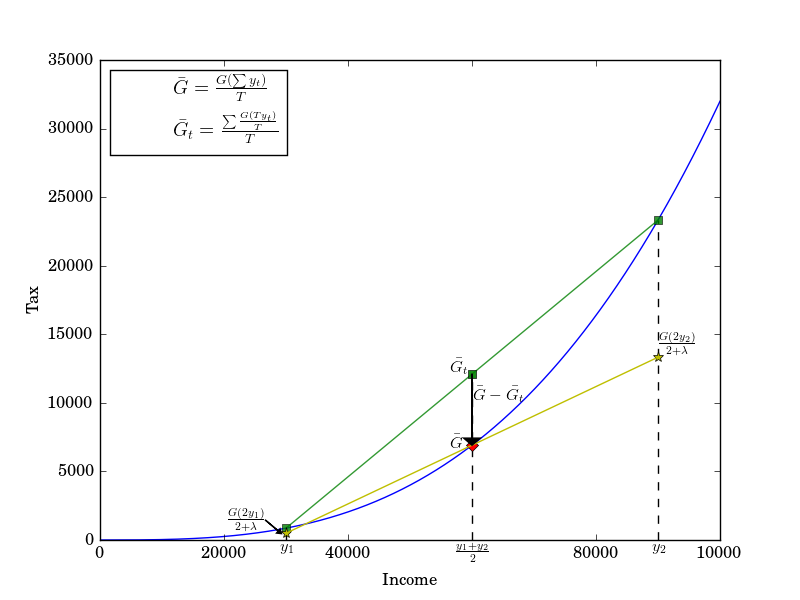
\includegraphics[width=1.0\textwidth]{./image_graph2.png}}
\end{figure}

We must observe that except the monthly equal tax, the total amount paid at
the end of the year to the treasury is the same for the other four tax
payments.\ The neutrality property essential to Vickrey is then satisfied by
the four taxation schemes. We must find other criteria to decide between them.
The well-being associated to them seems at least an important criterion.\ 

\subsection{Comparison of well-being for the tax regimes}

We first show that the annual well-being is higher with the monthly
compensated scheme than with the equal monthly scheme. The current system is
also dominated by the monthly compensated scheme. We end up with a comparison
with the Vickrey's proposal by means of simple examples.

\paragraph{Monthly compensated versus equal payment\medskip}

\newtheorem{mydef}{Theorem} \begin {mydef}
If the subutility is concave and the underlying annual tax schedule is convex, the intertemporal utility of the taxpayer over the yearly span
is higher with a monthly compensated scheme than with an equal split scheme.
\begin {equation}
\sum _{1}^{T}{u_t\left (y_t-\cfrac {G\left (\sum {y_t}\right )}{T}\right )}\leq \sum _{1}^{T}{u_t\left (y_t-\frac{G(Ty_t)}{T+\lambda }\right )}
\end {equation}
\end {mydef}


\begin{proof}
We check that the conditions of the dominance theorem are satisfied. Clearly
because both systems are neutral to the earning timing within the year, the
sum of the monthly disposal incomes is the same with the two systems.\ Now we
have to check that the partial sums of monthly tax amounts are lower with the
monthly compensated scheme than with the equal payment regime, implying that
we have the reverse relation for disposable incomes. It amounts to compare for
the first $k$ months which are reranked according to increasing gross income
order that:


\[
\sum_{t=1}^{k}\frac{1}{T+\lambda}G(Ty_{t})\leq\frac{kG(T\bar{y})}{T}
\]
with $\bar{y}$ the monthly mean. By definition
\[
T+\lambda=\frac{\sum_{1}^{T}G(Ty_{t})}{G(T\bar{y})}
\]
Substituting the value of $T+\lambda$ into the above expression we obtain%

\[
\frac{\sum_{t=1}^{k}G(Ty_{t})}{\sum_{1}^{T}G(Ty_{t})}G(T\bar{y})\leq
\frac{kG(T\bar{y})}{T}
\]
which simplifies in
\[
\frac{1}{k}\sum_{t=1}^{k}G(Ty_{t})\leq\frac{1}{T}\sum_{1}^{T}G(Ty_{t})
\]
which must be true because the partial average of $k$ increasing numbers is
always lower than the total average of the same $T$ numbers with
$T>k.$\end{proof}% \bigskip

The proof shows that the result is indeed stronger than the statement of the
theorem suggests.\ It indicates for instance that if the sequence of income is
increasing over the year, then all partial intertemporal utility streams
covering any sub-period starting from January are higher for the monthly
compensated tax scheme than for the equal payment regime.\ The taxpayer is
happier for any subperiod considered, the first $k$ months from $k=1,..,12.$

The general idea illustrated by \autoref{Utility side} is that the
compensation takes out the potential negative effect of paying more taxes with
a monthly tax base and the only remaining effect is the income smoothing.

\begin{figure}[ptb]
\caption{Utility changes with the Monthly compensating scheme}%
\label{Utility side}
{\centering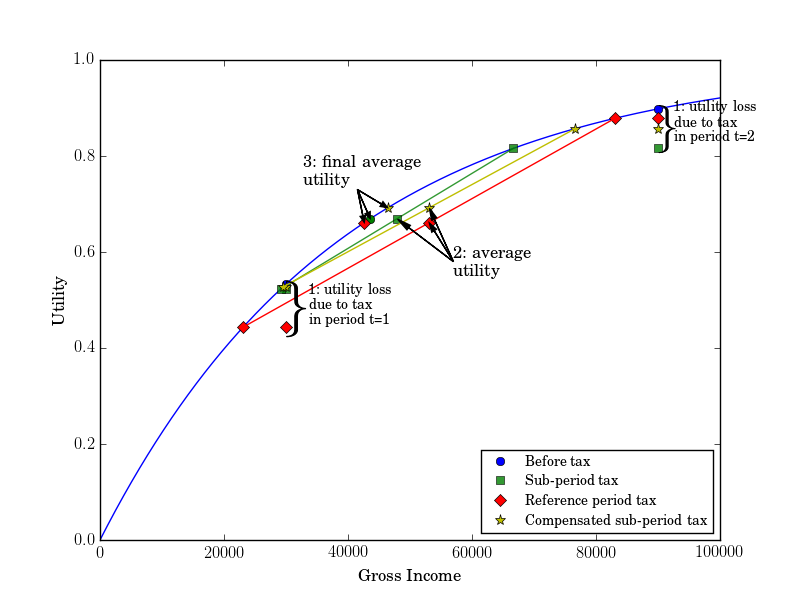
\includegraphics[width=1.0\textwidth]{image_graph3.png}}
\end{figure}

\paragraph{Monthly compensated versus current system}

For reasons that will appear in a transparent way in the next subsection, we
will compare both tax payments when the sequence of gross incomes is
increasing within the year.\ It should be the case for many full-time
employees with year-end bonuses.\ 

So let us consider the case where $y_{1}$ $\leq y_{2}\leq,....,\leq y_{12}.$

\begin{claim}
The monthly compensated system brings out higher welfare than the current
system for every subperiod starting from the first month, including the full
year.\ It brings also higher welfare for every month except may be December.
\end{claim}

The statement follows from the fact that $\lambda>0$ and the mathematical theorem.\ 

\paragraph{Vickrey versus Monthly compensated}

The Vickrey mechanism is backward looking. The monthly compensated is taking
advantage of knowing the full income stream. It is a bit unfair in some sense
to compare them since we compare a perfect information mechanism with a
mechanism which relies upon the updated information at each month.
Nevertheless, it is still interesting to understand in which situations the
Vickrey mechanism performs badly.\ We are considering simple cases which allow
us to develop the intuition for more complex situations. Comparing the two
mechanisms for more general income streams is not that simple since Vickrey
involves substractions and the monthly compensated scheme divisions. This
makes the comparision less trackable. There are cases where we cannot conclude
from a theoretical view point. \ 

\subparagraph{Two sub-periods}

We suppose that there exists two subperiods, $1$ and $T=2$.\ Either (first
case) $y_{1}>y_{2}$ or (second case) $y_{1}<y_{2}$. In both cases, $g_{1}%
^{MC}<$ $g_{1}^{V}$ implying that $g_{2}^{MC}>$ $g_{2}^{V}$ because the
cumulated taxes are the same.\ It suffices then to build on the mathematical
result to state that:

\begin{claim}
In case of an increasing income stream within the year, there will be a
welfare gain at each subperiod starting from the first month including the
full year to switch from the Vickrey mechanism to the monthly compensated one.
In case of a decreasing income stream, the opposite statement holds.
\end{claim}

\subparagraph{Three sub-periods}

Involving a third period in the framework introduces some intricacies.\ We are
able to compare both mechanisms by building upon the two-period case and
considering a variable income in the third and last period $T=3.$ We begin
with generalizing the previous claim about monotone income streams.

\textbf{Monotone income streams}

\textbf{\ }

\textit{Case 1 Increasing income streams} $y_{1}=y_{2}<$ $y_{3}$

We can think this situation as featuring a year-end bonus following a steady
income over the previous months.

The idea is always the same: to check that the conditions of the mathematical
theorem holds.\ 

It is still obvious that $g_{1}^{MC}<$ $g_{1}^{V}.\ $

We now have to look at the second partial sum and we prove that $g_{1}%
^{MC}+g_{2}^{MC}<$ $g_{1}^{V}+g_{2}^{V}$

By definition $g_{1}^{MC}+g_{2}^{MC}=\frac{1}{3+\lambda}[G(3y_{1}%
)+G(3y_{2})]=\frac{[G(3y_{1})+G(3y_{2})]}{[G(3y_{1})+G(3y_{2})+G(3y_{3}%
)]}G(y_{1}+y_{2}+$ $y_{3})$

Using now the fact that $y_{1}=y_{2}=y$ we obtain

$g_{1}^{MC}+g_{2}^{MC}=\frac{2G(3y)}{[2G(3y)+G(3y_{3})]}G(2y+$ $y_{3}%
)=\frac{\frac{2}{3}G(3y)}{[\frac{2}{3}G(3y)+\frac{1}{3}G(3y_{3})]}G(2y+$
$y_{3})$

On the other hand, $g_{1}^{V}+g_{2}^{V}=\frac{2}{3}G(\frac{3}{2}(y_{1}%
+y_{2}))=\frac{2}{3}G(3y)$

Therefore $g_{1}^{MC}+g_{2}^{MC}=\frac{g_{1}^{V}+g_{2}^{V}}{[g_{1}^{V}%
+g_{2}^{V}+\frac{1}{3}G(3y_{3})]}G(2y+$ $y_{3})$

Then the issue of $g_{1}^{MC}+g_{2}^{MC}<$ $g_{1}^{V}+g_{2}^{V}$ is equivalent
to $\frac{g_{1}^{V}+g_{2}^{V}}{[g_{1}^{V}+g_{2}^{V}+\frac{1}{3}G(3y_{3}%
)]}G(2y+$ $y_{3})<g_{1}^{V}+g_{2}^{V}$

Factorizing gives the following condition $(g_{1}^{V}+g_{2}^{V})^{2}%
+(g_{1}^{V}+g_{2}^{V})(\frac{1}{3}G(3y_{3})-G(2y+$ $y_{3})>0$

A sufficient condition is: $\frac{1}{3}G(3y_{3})>G(2y+$ $y_{3}).$

For a given $y,$ it is clear that due to the convexity of $y_{3},$ there
exists a cutoff point $y_{3}^{\ast}$ such that $G(3y_{3})>3G(2y+$ $y_{3})$

The following claim makes stock of the above reasoning

\begin{claim}
In case of an increasing income stream within the year, $y_{1}=y_{2}<$
$y_{3},$ for $y_{3}$ big enough, there will be a welfare gain at each
subperiod starting from the first month including the full year to switch from
the Vickrey mechanism to the monthly compensated one. By continuity it is true
for $y_{2}$ slightly larger than $y_{1}.$
\end{claim}

We shall keep in mind that we have the intuition that the result is more
general than that but now on we do not have a more general proof.

\ 

\textit{Case 2 Decreasing income streams }$y_{1}>y_{2}>$ $y_{3}=0$

This situation features the case of an individual which is employed in the
first part of the year, then become unemployed and receives the employment
benefits to end the year with no income. The increasing ranking of income
denoted $y_{\left[  i\right]  }$ is the opposite of the calendar ranking. That
is $y_{\left[  1\right]  }=y_{3},y_{\left[  2\right]  }=y_{2}$ and $y_{\left[
3\right]  }=y_{1}.$

It follows from the definitions that $g_{_{\left[  3\right]  }}^{MC}<$
$g_{\left[  3\right]  }^{V}$. We immediatly deduce that it must be true that
$g_{\left[  1\right]  }^{MC}+g_{\left[  2\right]  }^{MC}>$ $g_{\left[
1\right]  }^{V}+g_{\left[  2\right]  }^{V}$.\ To apply the mathematical
theorem, we must also have that $g_{\left[  1\right]  }^{MC}<g_{\left[
1\right]  }^{V}$ that is, $g_{3}^{MC}>g_{3}^{V}.$

Be definition we know that $g_{3}^{MC}=0.$ We must prove that $g_{3}^{V}<0.$

It goes back to the computation of $G(y_{1}+y_{2})-\frac{2}{3}G(\frac{3}%
{2}(y_{1}+y_{2}))$ which amounts to compare $\frac{3}{2}$ and $\frac
{G(\frac{3}{2}(y_{1}+y_{2}))}{G(y_{1}+y_{2})}$

If we assume in addition that $G(0)=0$, then convexity implies that
$G(\frac{3}{2}(y_{1}+y_{2}))>\frac{3}{2}G(y_{1}+y_{2}).\ $We can then state


\begin{claim}
Assume that $G(0)=0.$ In case of a decreasing income stream within the year, \hfill
$y_{1}>y_{2}>$ $y_{3}=0$ there will be a welfare gain at each subperiod
starting from the first month including the full year to switch from the
monthly compensated mechanism to the Vickrey one. By continuity it is true for
$y_{3}$ close to $0.$
\end{claim}


We have dealt with the case where $y_{3}$ is small or very large. It remains
to deal with the case of $y_{3}$ is between $y_{1}$ and $y_{2}.$ We will
consider the case where $y_{3}=\frac{y_{1}+y_{2}}{2}.$ Indeed, it is an
interesting case because it corresponds to the minimal value of $\lambda$ as a
function of $y_{3}$ for a given $y_{1}$ and $y_{2}$. It is when the correction
brought by the monthly compensated mechanism is minimal with respect to the
monthly mechanism.
\medskip

\textbf{Non-monotone profiles}

We are going to deal with two profiles, case 1\ where period 2 is the peak,
$y_{2}=Max(y_{1},y_{2}),$ and case 2 where period 2 is the dip, $y_{2}=Min$
$(y_{1},y_{2}).$

Case 1:\ Period 2 is the peak

Period 1\ is then the worst-off period for the taxpayer.\ By definition,
$g_{1}^{MC}<$ $g_{1}^{V}.$ The next poor period is period 3.\ Let us compare
the tax payment for this period. $g_{3}^{MC}=$ $\frac{1}{3+\lambda}%
[G(3y_{3})]=$ $\frac{1}{3+\lambda}[G(\frac{3}{2}(y_{1}+y_{2})]$

Now let us compute $g_{3}^{V}.$ $g_{3}^{V}=G(y_{1}+y_{2}+y_{3})-\frac{2}%
{3}G(\frac{3}{2}(y_{1}+y_{2}))=G(\frac{3}{2}(y_{1}+y_{2})-\frac{2}{3}%
G(\frac{3}{2}(y_{1}+y_{2}))=\frac{1}{3}[G(\frac{3}{2}(y_{1}+y_{2})]$

We conclude that $g_{3}^{MC}<g_{3}^{V}$ and therefore $g_{1}^{MC}+g_{3}^{MC}<
$ $g_{1}^{V}+g_{3}^{V}.$\ The second partial sum of taxes for monthly income
ranked in increasing order is lower for Monthly compensated scheme than for
Vickrey.\ We can then state

\begin{claim}
When $y_{1}<y_{3}=\frac{y_{1}+y_{2}}{2}<y_{2}$, the taxpayer is better of with
the Monthly compensated scheme than with the Vickrey mechanism and this is
true for any subperiod starting from the first month including the full year.
\end{claim}

Case 2: Period 2\ is the worst-off period.

By definition, period 1\ is the best-off period and it turns out that
$g_{1}^{MC}<$ $g_{1}^{V}.$ We derive that $g_{2}^{MC}+g_{3}^{MC}>$ $g_{2}%
^{V}+g_{3}^{V}.$

From the previous derivation of the above claim, we know that $g_{3}%
^{MC}<g_{3}^{V}.$ Therefore, it must be that $g_{2}^{MC}>g_{2}^{V}$. Then the
conditions of the theorem applies to the benefit of the Vickrey mechanism.\ 

\begin{claim}
When $y_{2}<y_{3}=\frac{y_{1}+y_{2}}{2}<y_{1}$, the taxpayer is better of with
the Vickrey scheme than with the Monthly compensated mechanism and this is
true for any subperiod starting from the first month including the full year.
\end{claim}

It appears that there is no global winner nor looser when comparing Vickrey
and the Monthly compensated mechanism.\ The discussion below will pave the way
to hint that the income configuration when the Monthly compensated mechanism
dominates are those for which the taxpayer appears as the most constrained by
the imperfect financial market.\ 

\subsection{Discussion}

We will discuss five points.\ The first two are related to a less crude
representation of preferences of individuals.\ They care about consumption and
leisure and they adapt their behavior to the tax changes.\ We introduce them
in the analysis in turn.\ We then discuss the negative income tax, the
convexity assumption of the tax schedule and the implementation of the monthly
compensated tax scheme.\ 

\paragraph{Borrowing and saving}

If an individual can fully borrow or save within a year, then it is clear that
what matters is the total disposable income over the year. The four systems
are then equivalent in terms of consumer welfare and the discussion vanishes,
except that we can say that with the monthly compensated schedule, the need of
precautionary saving weakens since the profile of disposable income displays
less variability than with the current system. Our results are worth it for
individuals with no or very small saving. It is then a result that can be
useful for developing countries and that matters much for poor households in
rich and developed country. It is common for poor household that the beginning
of the month is easier than the end because they have spent most of their wage
or their social welfare benefits during the month (see \citet{hastings2010first}).

We can extend the validity of our results in a framework when the household
can save but not borrow (or at a much higher rate).\ We will prove below that
we are back to the framework that we have considered above.\ We will prove it
on the basis of a simple example with two periods and a zero interest rate.

Let us call $c_{1}$ and $c_{2}$ the consumption levels for these two periods.
What matters for the household is the intertemporal utility of consumption
streams $U=u(c_{1})\,+u(c_{2}).\ $We will look at the expected utility denoted
$E(U)$ at the beginning of the year when the taxpayer does not know what would
be the income stream during the year.\ 

\ There are two cases.\ In the first case where $y_{1}>y_{2}$, the individual
can save in the first period and then the optimal equal consumption plan
between the two periods can be achieved.\ In that regime, the consumption in
each period is given by the average income over the year, that is, for the
full year we get $2u(\frac{y_{1}+y_{2}}{2})$ as the annual utility.\ In the
second case where $y_{1}<y_{2},$ the individual cannot borrow and then the
consumption of her first period is constrained to be $c_{1}=y_{1}$ and the
consumption of the second period is then $c_{2}=y_{2}$. Therefore, the
intertemporal utility is given by $u(y_{1})+$ $u(y_{2}).$

Combining both elements and introducing the probability of the two events, the
expected utility reads:%

\[
E(U)=\Pr(y_{1}<y_{2})[u(y_{1})+u(y_{2})]+\Pr(y_{1}>y_{2})[2u(\frac{y_{1}%
+y_{2}}{2})]
\]


The above theorems are related to the first part of the expected utility,
$[u(y_{1})+u(y_{2})]$.\ The second part of the expected utility is constant
for the four tax schemes in discussion.\ We conclude that the results remain
valid when the taxpayer is not allowed to borrow at the same conditions as she saves.

Provided that the consumer starts the new year with almost no saving -- which
occurs in the US\ at least for the average people in the bottom quintile -- an
increasing income sequence within a year is a sequence where the absence of a
perfect capital market bites the most. It is the case where the individual
will benefit the most of consumer credit since by assumption it cannot draw on
her precautionary savings. It is here when the monthly compensated system will
help and we recall that, in these circumstances, it dominates the Vickrey
mechanism.\ Of course, the reasoning depends on the assumption that the
accounts are cleared at the start of the year which can be viewed as an hoc
assumption. Here, we are in some sense trapped by the annual fiscal framework.

We do not introduce a monthly discount rate in the intertemporal utility. The
monthly discount rate will be very low if any and it can be argued that many
people have a spending behavior as if they have a higher marginal utility in
let say December, July and August than in March or November.\ A low discount
rate will not be enough to invalidate the above results.\ It will just make
the results more difficult to prove.

\paragraph{Labor supply}

We already argue in the introduction that caring about the variability of
earnings within a year does make sense if this variability is not the result
of a choice. We can easily think of situations where the individual prefers to
some extent to gather her hours of work rather than spreading them out.\ The
summer vacations are an example of corner solutions for leisure.\ Many
professors prefer to concentrate their teaching duties on one semester.\ Many
pilots and stewarts also prefer to travel with little rest for a while
followed by a long period of leisure.\ The same goes for seasonal workers in
seaside or ski resorts. Even if the change of the tax base does not stem from
the fact we wish to improve the situation of these individuals, it is
important to check that the new tax configuration will not have adverse effect
on their behavior and welfare.

The utility will be of the form $U(c+v(l))$ with $v$ can have some convex
parts, in such a way that the individual is choosing a corner solution.\ For
instance take the case of US\ university professors with a 9 month contract.
Does the monthly compensated system will make them more inclined to accept a
work during the summer?

The answer is not obvious and depends on their knowledge of the tax system. We
will say that people are myopic if they only look at the monthly marginal tax.
The monthly marginal tax rate will be lower with the monthly compensated
system than with the current system.\ TConsequently, the substitution effect
will pushed toward working more each month! As illustrated in Figure 1, the
decrease of marginal tax rates will be higher for very active months than in
rather inactive months.\ By definition, the income effect would be zero. So we
conclude that in the myopic case, people will work more each month and even
more the loaded months.\ Now, it is also possible that the rational university
professor will only contemplate the annual tax schedule which has not changed
by definition and then decide not to change her behavior. In all cases, we
expect that the magnitude of the behavioral reaction will be small if the
actual choice is a corner solution.

\paragraph{Negative income tax}

The results were obtained for an income tax which does not include transfers
and benefits. The case of a negative income tax can be analyzed along the same
lines and all the results hold. The main difference is that $\lambda$ is now
negative.\ Indeed we still have
\[
\sum_{1}^{T}\frac{G(Ty_{t})}{T}\geq G(\sum_{1}^{T}y_{t}))
\]
but assuming that $G(Ty_{t})$ and $G(\sum_{1}^{T}y_{t}))$ are negative, the
value of $\lambda$ which will make both sides of the inequation equal is
negative (or alternatively we will have $T-\lambda$ with $\lambda>0)$.%

\[
\sum_{1}^{T}\frac{1}{T-\lambda}G(Ty_{t})=G\left(  \sum_{1}^{T}y_{t}\right)
\]


In the similar figure as Figure 1, the chord will be always above the function
since the tax schedule remains convex.\ However the amount of benefits
transferred to poor people are now lower with the monthly compensated tax than
with the equal payment system. We then have to adjust with a negative
$\lambda$ and it turns out than the poor months will be more heavily
subsidized than the months when the incomes are higher because the gap
\[
\frac{1}{T-\lambda}G(Ty_{t})-\frac{1}{T}G(Ty_{t})=G(Ty_{t})(\frac{\lambda
}{\left(  T-\lambda\right)  T})
\]
will be the higher the tax amount $G(Ty_{t})$ is far from 0, meaning that $t$
is a bad month.\ The smoothing effect of the monthly compensated tax will
still operate and the results remain valid in the benefit side as well as in
the tax side.

\paragraph{Convexity}

We assume from the outset that the tax schedule is convex. Many applied works
have shown that the effective marginal tax is in fact decreasing on the bottom
part of the income distribution in many countries because of the phasing out
of the benefit system.\ In some cases, \citet{diamond1998optimal} has shown
that the static optimal marginal income tax rate should follow a U-shape, a
feature also observed in many countries (see \citet{diamond2011case} and
\citet{mankiw2009optimal}.)\ It adds an additional layer of complexity and it
is difficult from a theoretical view point to figure out whether adopting the
monthly compensating scheme will be good or harmful for the taxpayer welfare.
It militates for empirical studies and it is what we are doing in the next
section. The only thing that we can add is that on the income range for which
the marginal tax rate will be decreasing, switching to a monthly compensating
scheme will be harmful for benefit recipients. The proof of this statement
works exactly on the same way as the proofs or our results.\ By the way, it is
not fully sure that in a dynamic context with poverty traps and risk the
subsidization of earnings should phased out at a relatively high rate

\paragraph{Implementation}

On those 4 tax schemes, only the current and the Vickrey system are
implementable on the spot taking account the monthly available information.
The equal payment and the monthly compensated tax needs for the government to
foresee incomes before their realisation. If it is indeed impossible to do it
without error, it is possible for the tax authorities to forecast the current
variability of income for each taxpayer or for each taxpayer type. Indeed we
think that a local analysis can be performed to compute the adjustement
parameter, $\lambda,$ as a function of the degree of convexity of the taxation
scheme (the relative Arrow-Pratt degree of risk loving, $\frac{G^{"}%
(y)}{G^{\prime}(y)}y$) and a measure of risk, the standard deviation or the
coefficient of variation. Once the formulae will be established, it remains to
estimate the within-year SD for different types of taxpayers.\ The available
information will be the past information that the tax authorities have, the
characteristics of the taxpayer (education, type of job, sector, gender, age
etc.) and why not the information that the taxpayer will be able to provide
about the variability of income she foresees for the coming year.\ An
individual forecasting error will be made for sure, but the good thing will be
that the (positive or negative) adjustment at the end of the fiscal year will
likely be much less big than it is actually.\ It means that in average the tax
payment will be more accurate each month than now.\ An exploration on actual
data is then needed to evaluate the heterogeneity dimension of taxpayers in
terms of the adjusment parameter $\lambda.$ This is the purpose of the next sections.

\section{Data \& French tax system}

We first give some information about the French tax system and compare it to
some other systems.\ We then move to the data and show an estimate of the
between-month variabilility.

\subsection{Tax Schedules: From theory to practice}

In the theoretical section, the general shape of $G$ was very general and
stated to be convex for the welfare gains results. Obviously the precise shape
of the tax function would be of primary importance for the matter discussed,
weather in terms of gain or loss, and even in a more significant way for the
size of the gains. $G$ could be seen as a specific tax such as income tax or
as the effective tax (i.e the sum of all taxes and benefit one is entitled).
Even though effective taxation is the salient point for public economist to
work on, it should be clear that since all taxes are not based on the same
temporality, a static view point can overwrite some information and can lead
to misleading conclusions. We see as as first step to focus on a simulation
which only involves the income tax schedule.\ 

\paragraph{Piecewise linear tax scheme}

Most countries (to the notable exception of Germany) have piecewise linear
income tax schemes.

A piecewize linear tax scheme is defined as a sequence of (usually) increasing
marginal tax rate, \footnote{as defined in P.J. Lambert \emph{The distribution
and redistribution of income, third edition} P.181}:%

\[
0 < m_{0} < m_{1} < ... < m_{p}
\]
and a sequence of thresholds specifying the bands of taxable income to which
the respective rates apply.
\[
0 = \beta_{0} < \beta_{1} <...< \beta_{p}
\]


If $y \in[\beta_{k}, \beta_{k+1}] $, then the tax liability is :%

\[
s(y) = \sum_{j \leq k -1} m_{j}(\beta_{j+1} - \beta_{j} ) + m_{k} (y -
\beta_{j} )
\]


It is clear that if one's income stays between two tax brackets, the taxpayer
is comparable to one facing a flat tax, and all the characteristics concerned
by the above paragraph still holds. So with a piecewise linear tax scheme, one
would need to have large enough variation in income to be concerned by a
change in tax frequency concerning the amount paid.

\paragraph{France tax system}

France has an annual income tax that most taxpayers pays on a monthly basis
(one tenth of the tax based on last year income for most fiscal household).
\footnote{In fact, there is several systems among which the taxpayer can
choose. A three-time payment of the tax (in February, May, and September), a
monthly payment of the tax, or a monthly payment of the tax consisting of 10
payments from January to October that correspond to one tenth of last year due
tax. If the due income tax is greater for one year than the preceding year,
additional payment are required in November and December. More than two-thirds
of households choose that later option.} It consists of a tax applied to a
fiscal household. A fiscal household is an entity based on family situation:
married couples or under civil union\footnote{\textit{Pacte civil de
solidarit\'{e}} (Pacs)} will constitute one unit, single constitutes one
fiscal household and couples without civil union will form two fiscal households.

France Income tax consists of a piecewise linear tax scheme composed in 2009
of 5 tax brackets.

\begin{table}[ptb]
\caption{France 2009 Income Tax Schedule}
%descrptive_statistics-new_monthly_2 12/06/2017 [31]
\centering
\resizebox{8	cm}{!}{\begin{tabular}{|c|c|}
\hline
from 0 to 6011 euros & 0\%\tabularnewline
\hline
from 6011 to 11991 euros & 5,5\%\tabularnewline
\hline
from 11991 to 26631 euros & 14\%\tabularnewline
\hline
from 26631 to 71397 euros & 30\%\tabularnewline
\hline
from 71397 to 151200 euros & 41\%\tabularnewline
\hline
beyond 151200 euros & 45\%\tabularnewline
\hline
\end{tabular}}\end{table}


Thus in the formalised version of the piecewise linear tax scheme 
\begin{itemize}
\item[•] $\vec{m} = [6011, 11991, 26631,71397, 151200]$,  and, 
\item[•] $\vec{\beta} = [0, 5.5, 14,30, 41, 45]$
\end{itemize}
\medskip 

To compute tax liability, for a single without kid we just have to apply
taxable income to the tax scheme.%

\[
\text{Final tax} = G( \text{taxable income}) = \sum_{j \leq k -1} m_{j}%
(\beta_{j+1} - \beta_{j} ) + m_{k} (y - \beta_{j} )
\]


Joint taxation consist of a system called \emph{fiscal shares}
\footnote{\emph{Parts fiscales} in French}. A certain number of fiscal shares
are attributed to each fiscal household based on its composition: 1 share for
a single, two shares for a couple under civil union. Then each dependent child
gives additional shares: 0.5 for each two first childs, 1 share for each child
after the second one.\footnote{There exists a certain number of exceptions and
special case, single parents benefit from an additional half-fiscal share,
there exist specific rules for disable people, etc.} We then divide taxable
income by the number of fiscal shares and we refer to it later on as
normalized tax base. The piecewise linear scheme is then applied to the
normalized tax base and finally the obtained amount is multiplied by the
number of fiscal shares to obtain the tax liability.

\begin{dmath*}
\text{Final tax} = G \left( \frac{ \text{taxable income}}{ \text{ fiscal shares}} \right) \times \text{fiscal shares} = \sum_{j \leq k -1} m_j(\beta_{j+1} - \beta_j ) + m_k \left(\frac{y}{\text{fiscal shares}} - \beta_j \right) \times \text{fiscal shares}
\end{dmath*}


There exists also a mechanism called \emph{la d\'{e}cote} which is a tax break
for household paying a small amount of tax. This mechanism doubles the
marginal tax rates in the two first brackets. It does not take family
situation into account appart from being in couple or not. This mechanism
introduces a non-convexity in the tax schedule.\ Another source of local
non-convexity is that for a tax due lower than \euro62 the taxpayer does not
have to send a check to the tax authorities.\ 

France has also many benefits that mainly concerns households exempted to the
income tax, and that do not have a smooth or convex shape of the effective MTR.

\begin{figure}[ptb]
\caption{2009 French Income Tax, and Individual Income Distribution.}%
\label{fig:distrib_and_rates}
%article_graphs_simulation_results-new_monthly 20/05/2017 [65]
\par
\begin{center}
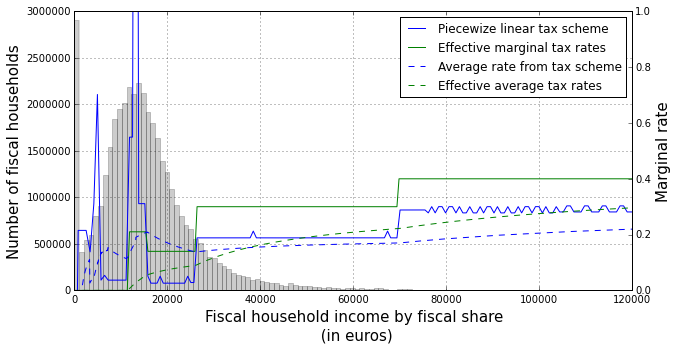
\includegraphics[width=\textwidth]{fiscal_household_income_distr_with_rates.png}
\end{center}
\end{figure}

As we can see on \autoref{fig:distrib_and_rates}, on the range \euro10,000 to
\euro30, 000, there are 4 tax brackets where there is only 2 from \euro30, 000
to \euro120, 000. With the introduction of benefits to this analysis and their
high number into the analysis, the number of tax-brackets soar at the very
bottom of the distribution as we can see on \autoref{fig:distrib_and_rates}
effective MTRs (which is for single individuals). The inclusion of family
support benefits, local taxation, "social tariffs" for telephone and
electricity utility services, Universal Health Care Cover, etc, would even
make the picture more complicated. \footnote{See \citet{anne2012rsa} for more
information about the diffent benefits (monetary or in kind) depending of the
administrative level.}

\paragraph{External Validity}

France has thus many benefits that imply non-convex effective MTR, and income
tax that embodied a tax break increasing the MTR at the beginning of the
income tax. It is the case for most OECD countries. For instance US has EITC
that increase marginal tax rate at the beginning of the piecewise tax scheme.
UK has also a working tax credit and income support that gives decreasing
marginal tax rate at the beginning of the income distribution. Both UK, and US
also have means tested benefits with phasing out implying high effective MTR,
and diminishing MTR. Thus as in France, households in UK and US are likely to
face both locally concave or convex effective tax schedule. Even if the labor
market and tax institutions of every country are specific, we believe that
some of the conclusions of our simulations for France can be extended to other
OECD countries.
\newpage



\begin{figure}[H]
\caption{UK scheme from \citet{brewer2010means} .}
\begin{center}
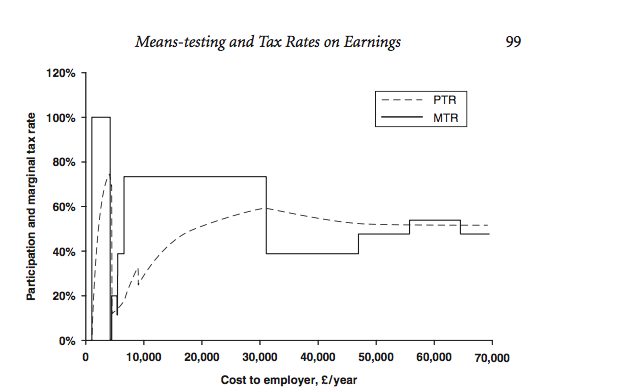
\includegraphics[width=\textwidth]{saez_brewer_shephard.png}
\end{center}
\end{figure}

\begin{figure}[H]
\caption{2004 US tax scheme from \citet{eissa2008redistribution}}
\begin{center}
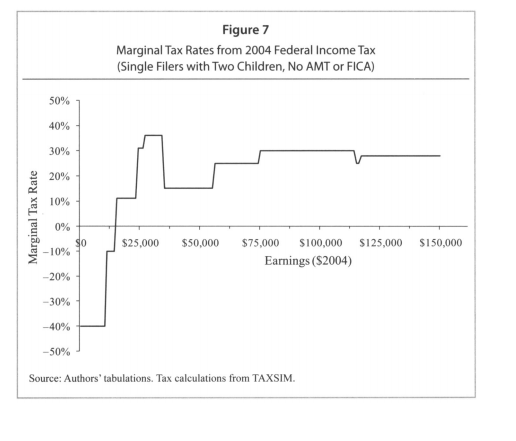
\includegraphics[width=\textwidth]{MTR_us_2004.png}
\end{center}
\end{figure}
\newpage


\subsection{Descriptive statistics}

To our knowledge, France does not have yet available database that allows for
the monitoring of the income tax at a monthly scale. We dodge that difficulty
by resorting to an administrative database which coupled detailed information
on the labor force and tax files.\footnote{The official name of the survey is
\emph{enqu\^{e}te sur les revenus fiscaux et sociaux} (ERFS)} We here explain
how we infer monthly income from French labor survey matched with tax returns.
Our attempt to deal with the earning time scale can to some extent be compared
to the practices in the British Household Panel Survey (see \citep[p. 4-5]{jenkins2000current}).

From the labor force survey, we have individual declared income by categories
over the year. Work related categories are labor income, unemployment income,
and retirement income. We have for each individual its monthly situation
(employed, unemployed, retired, student, inactive).

In order to infer a monthly income for each individual, we equally split
income-tax returns into the months for which an individual was in the
corresponding category. For example, employment income is allocated to months
where the individual was declared employed, unemployment income to months
where the individual was unemployed, and retirement income to the months where
the individual was retired. If an individual declares for a given month that
she was a student or inactive, the inferred income is zero. Other incomes
(capital incomes, etc) are equally split over the year. .

Without saying, our method is far from perfect. For those reasons, descriptive
statistics and results of the simulations should be taken with a piece of salt
and just as a rough estimation of the impact of a change of the tax system
toward a monthly compensated tax. In following sections, except when
specified, the observations are weighted such that it represents French
population in 2009. Technical details concerning the method are in the appendix.

\paragraph{Income Distribution and Variations Over Months}

\begin{figure}[ptb]
\caption{Aggregate Disposable Income by Months.}
\label{fig:aggreagate_income}
%descrptive_statistics-new_monthly_2 20/05/2017 [78]
\centering
%\hspace{-3.5cm}
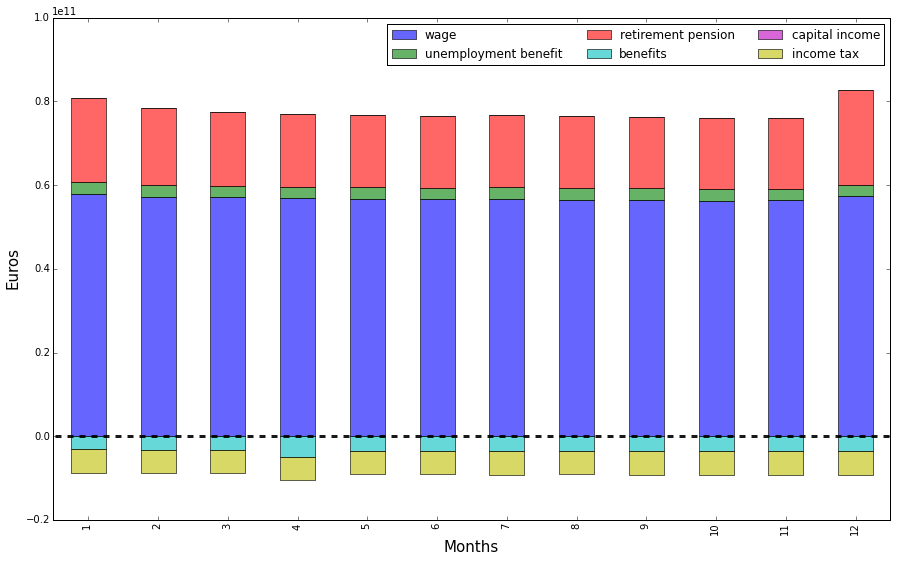
\includegraphics[width=\textwidth]{aggregate_income_by_month.png}\end{figure}

\autoref{fig:aggreagate_income} shows aggregate income per month, that is of a
bit more than \euro60 billions. The sources of income are steady, to the
exception of November due to a higher number of declared retired persons in
November 2009 in the French labor survey\footnote{Usually, retirement takes
place in September and they can be a delay between the retirement date and the
month when the person receives her first pension benefit.\ }%
.\autoref{fig:status_transition_simplified} represents a simplified version of
the possible transitions, such that taking a job that we define as not having
a work activity last month to having a work activity on the concerned month.
Job loss is defined as switching from being employed to unemployed, student or
inactive. Retirement is defined as switching from employed or inactive to
retired. \footnote{Since we have 5 types of situation (employed, unemployed,
inactive, retired, student), we can thus have $5\times(5-1)=20$ different
types of transition.We simplify here those transitions into 3 categories to
have a clearer view of the transitions. A more complete description of the
transitions are provided in the appendix.} \medskip

\begin{figure}
\caption{Aggregate Monthly Transitions}%
\label{fig:status_transition_simplified}
\begin{center}
%\hspace{-2.5cm}
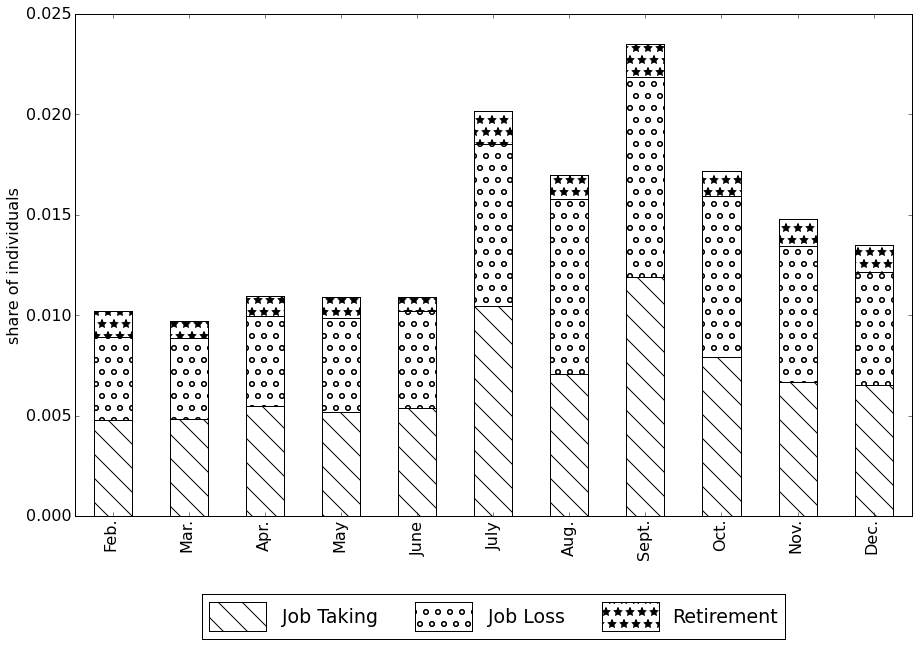
\includegraphics[width=\textwidth]{passage_barplot_simplified_proportions.png}
\end{center}
\end{figure}

We see that on average 1.4 \% of the individuals has a change of situation
each month. From those 1.4\%, 44\% are job losses, 48\% are job taking, and 8
\% are people that get retired.

\begin{table}
\caption{Share of Type of Transitions}%
\label{table}
%data cleaning monthly basis 13 new monthly 20/05/2017 [188] Table share of type of transition
\centering
\begin{tabular}
[c]{lcccccccccccccccccc}%
\toprule \addlinespace[5pt] Job loss & Job taking & Retirement 
 \\
\cmidrule(r){1-3} \addlinespace[5pt] 44\% & 48\% & 8\%  \\
\bottomrule
\end{tabular}
\end{table}

\begin{figure}
%data cleaning monthly basis 13 new monthly 20/05/2017 [186]
\par
\begin{center}%
\begin{tabular}
[c]{lrrrrr}%
\toprule {} & No Variation & Job Taking & Retirement & Job Loss & Sum of
Variations\\
\midrule Feb. & 79609 & 381 & 102 & 328 & 811\\
Mar. & 79646 & 384 & 66 & 324 & 774\\
Apr. & 79547 & 434 & 80 & 359 & 873\\
May & 79553 & 411 & 84 & 372 & 867\\
June & 79552 & 427 & 57 & 384 & 868\\
July & 78832 & 823 & 128 & 637 & 1588\\
Aug. & 79076 & 561 & 95 & 688 & 1344\\
Sept. & 78575 & 937 & 127 & 781 & 1845\\
Oct. & 79062 & 626 & 100 & 632 & 1358\\
Nov. & 79248 & 530 & 106 & 536 & 1172\\
Dec. & 79350 & 516 & 104 & 450 & 1070\\
Total & 872050 & 6030 & 1049 & 5491 & 12570\\
\bottomrule &  &  &  &  &
\end{tabular}
\end{center}
\end{figure}

%\autoref{fig:max_variation} represent the cumulative distribution function of individuals maximum variation of income within the year (the difference between lowest and highest income.
%With the assumptions we made 89 \% have a constant income over the year, and 11 \% of individuals have a variation of income within the year.
%\footnote{Those statements do not takes into account rise in salary or other type of variations except from those due to a change within unemployment, inactivity, retirement and employment.}
%
%\begin{figure}[H]
%\begin{center}
%\caption{Infra-annual Variation of Income.}
%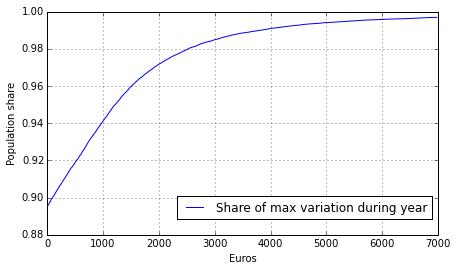
\includegraphics[width=\textwidth]{share_of_max_variation_old_2.png}
%\label{fig:max_variation}
%\end{center}
%\end{figure}


\autoref{fig:max_variation} represents the CDF of individual maximum variation
of income within the year (the difference between lowest and highest income).
With the assumptions we made, 86 \% have a constant income over the year, the
remaining share having a variable income. 5 \% has a variation that is higher
than 2000 euros. After some data cleaning to remove most obvious cases of bad
correspondence between income and status, we obtain less impressive variations
as in \autoref{fig:max_variation_cleaned}, where only 2 \% has an income
variation over \euro\ 1000.
        

\begin{figure}[ptb]
\caption{Infra-annual Variation of Income.}%



\begin{center}
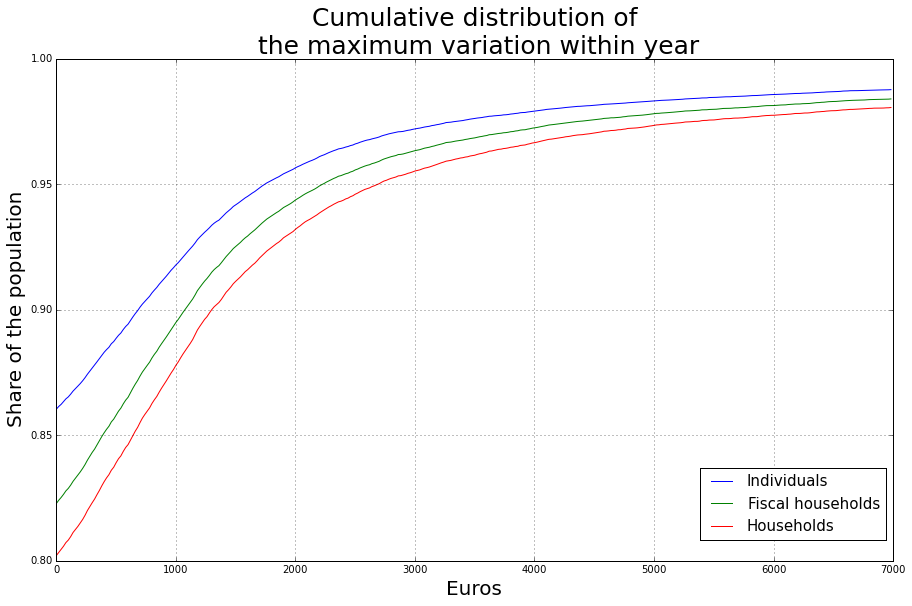
\includegraphics[width=\textwidth]{share_of_max_variation.png}
\label{fig:max_variation}
\caption{Infra-annual Variation of Income Corrected.}%
\label{fig:max_variation_cleaned}
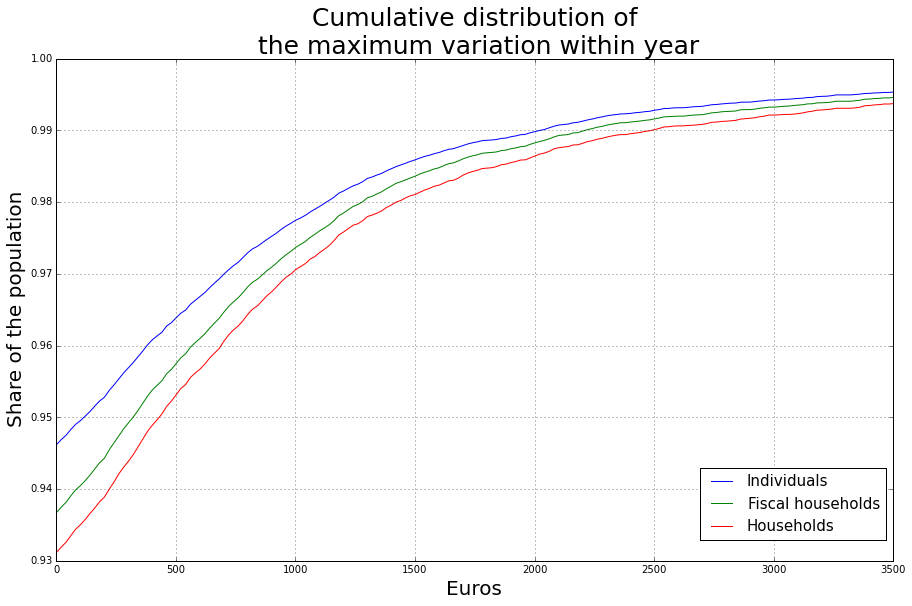
\includegraphics[width=\textwidth]{share_of_max_variation_cleaned.png}
\end{center}
\end{figure}



We can see that a significative share of individuals face a variation in
income during the year. The French tax system being piecewise linear, a change
in income does not necessarily mean a change in the tax amount since a fiscal
household would have to change of tax bracket to face a difference in the tax
amount. Joint taxation also takes its part on that dimension since it is the
average of incomes that are applied to the tax scheme. \footnote{More
precision on the joint taxation system in France in appendix}



\autoref{fig:variation_20} shows that most population concerned by
between-month income variation is at the bottom of the distribution, where the
income tax scheme is concave. \autoref{fig:variation_20} shows the share per
decile of people that have more than 20\% of income variation between the
worst month and the best month. \footnote{Here the graphs do not change much
after data cleaning.} The income limits of deciles are showed on the
horizontal axis in terms of normalized tax base. The MTR represents the MTR of
a tax-unit composed by one individual. The 22.5 \% MTR spike at the beginning
of the income range is due to a tax break called \emph{"la d\'{e}cote"} and
that --similarly to EITC-- creates diminishing MTRs at the beginning of the tax-schedule.

\begin{figure}[ptb]
\caption{Share per decile of individuals having more than a 20\% gap between
the worst month and the best month. .}%
\label{fig:variation_20}
%article_graphs_simulation_results-new_monthly 20/05/2017 [71]
\par
\begin{center}
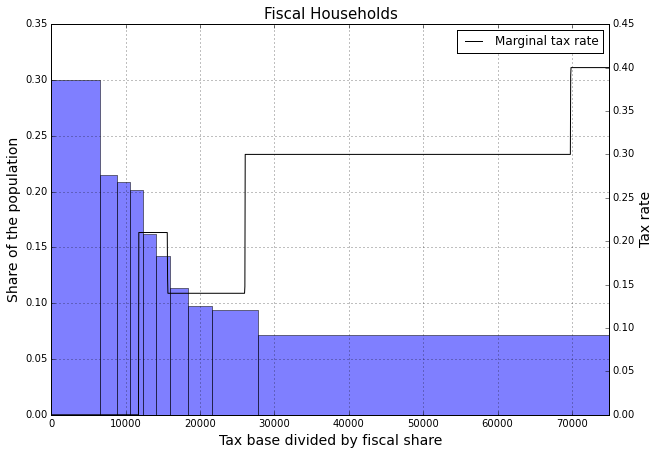
\includegraphics[width=\textwidth]{share_of_variation_20.png}
\end{center}
\end{figure}

We see that 10 \% of the population face the 30\% marginal tax bracket or a
higher marginal tax. If we assume that those tax-units do not move drastically
their month-to-month income (from one tax bracket to an other), it means that
most tax-payers in the last decile will likely face a flat-tax scheme.
However, the other 90\% of the population do not face a convex tax scheme:
they might pay less tax with a monthly payment! Moreover those having the
smallest income are the one that are the most likely to have variations in
income. Thus the poorest are the one facing the most risky labor demand, and
those variation are large enough to change the tax bracket they face.

These populations are also on average negative savers as showed by
\autoref{fig:saving_rate}. Thus marginal propensity to consume is very high
for those populations. The focus group faces most variation and poor savings.
This population also faces the highest number of potential tax backets, and
thus potential effects of disposable-income variation.

\begin{figure}
\caption{Mean saving rate by decile (French household family survey).}%
\label{fig:saving_rate}
\begin{center}
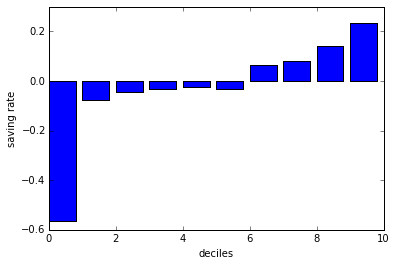
\includegraphics[width=\textwidth]{mean_saving_rate_by_decile.png}
\end{center}
\end{figure}

\section{Simulations}

We are performing a simulation exercice where the benchmark is the equal
payment system who will face three challengers, the Vickrey system, the
monthly system and the monthly compensated system.\ 

\paragraph{Simulation Hypothesis}

We use the microsimulation software \emph{OpenFisca} \footnote{Openfisca
registers many intricacies of the French tax system. The drawback is that so
far the calibration to macro data is not very accurate.
\par
\url{http://openfisca.org/en/} } to simulate a increase in the frequency of the tax from an annual to a
monthly one. We did that by changing all the tax formulas by making them
working on a monthly period instead of an annual one, multiplying all the
inputs by 12, and dividing the output by 12. Details and the code of the
reform are available on GitHub.

Switching from the actual system (that has many complexities that will not be
described here) to a monthly system without compensation increases the
simulated income tax revenues from 48 billion euros for 2009 to 54 billions.
To put the income on a monthly basis would generate a gain for the Treasury of
6 billion euros.

We then calculate the compensating term $\lambda$ for each household. 53\% of
the sample has a $\lambda$ equal to 0, 93 \% is very close to zero
($\mid\lambda\mid<0.001$). This difference between those two numbers is mainly
explained by small rounding differences (usually a cent of euro). We represent
the distribution of $\lambda$ on \autoref{fig:lambda_weighted}, $\lambda$s
equal to zero are taken out for a matter of scale. We see on
\autoref{fig:lambda_weighted} that a small part of the $\lambda$ are negative.
This is due to the non convex part at the beginning of the tax scheme.

\begin{figure}
\caption{$\lambda$ Distribution }%
\label{fig:lambda_weighted}
%article_graphs_simulation_results-new_monthly [74] 30/05/2017
\par
\begin{center}
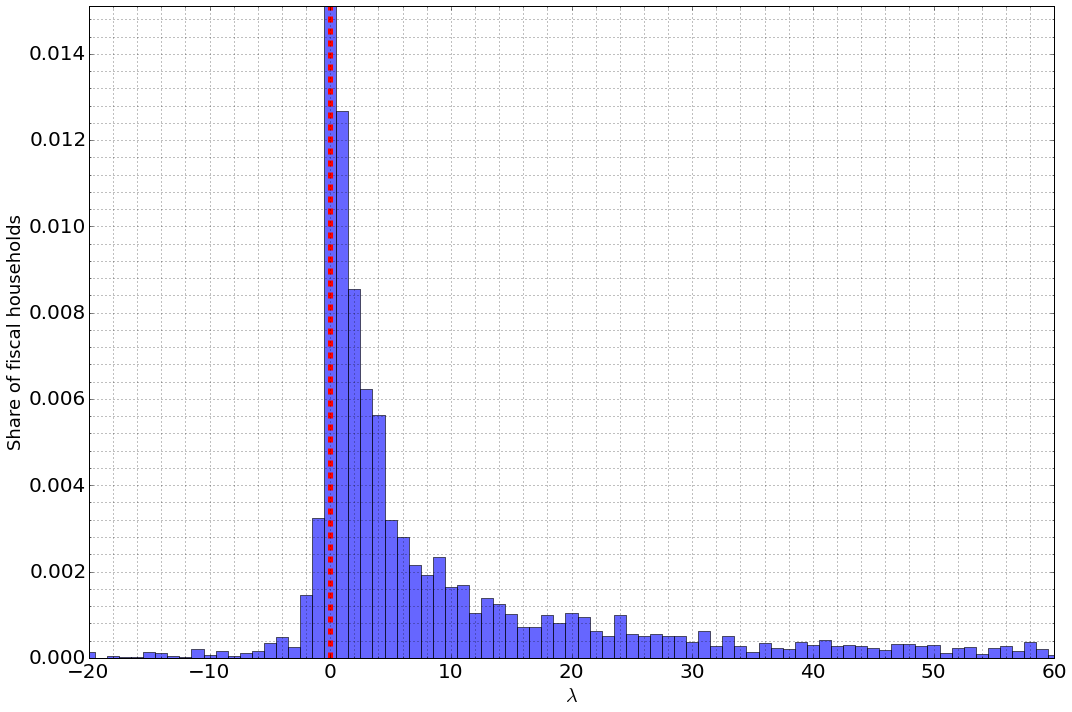
\includegraphics[width=\textwidth]{lambda_weighted.png}
\end{center}
\end{figure}

One should note that the French income tax being piecewise linear, having
income that varies is not sufficient for a change in the income tax. One would
need to change tax bracket in order to change the income tax with a monthly
basis. French tax schedule having quite large and few brackets, one would need
big variation in income in order to observe a significant difference. It is
even more true that France has a joint taxation (which double the length of
the tax brackets).

To summarize, we could say that a significative part (around 7 \%) of the
population would face a variation of their income tax if it is put on a
monthly basis.

\paragraph{Winner/Losers.}

\begin{figure}
\caption{ Winners and Losers with Monthly Tax. }%
\label{fig:monetary_winner_loosers}
\begin{center}
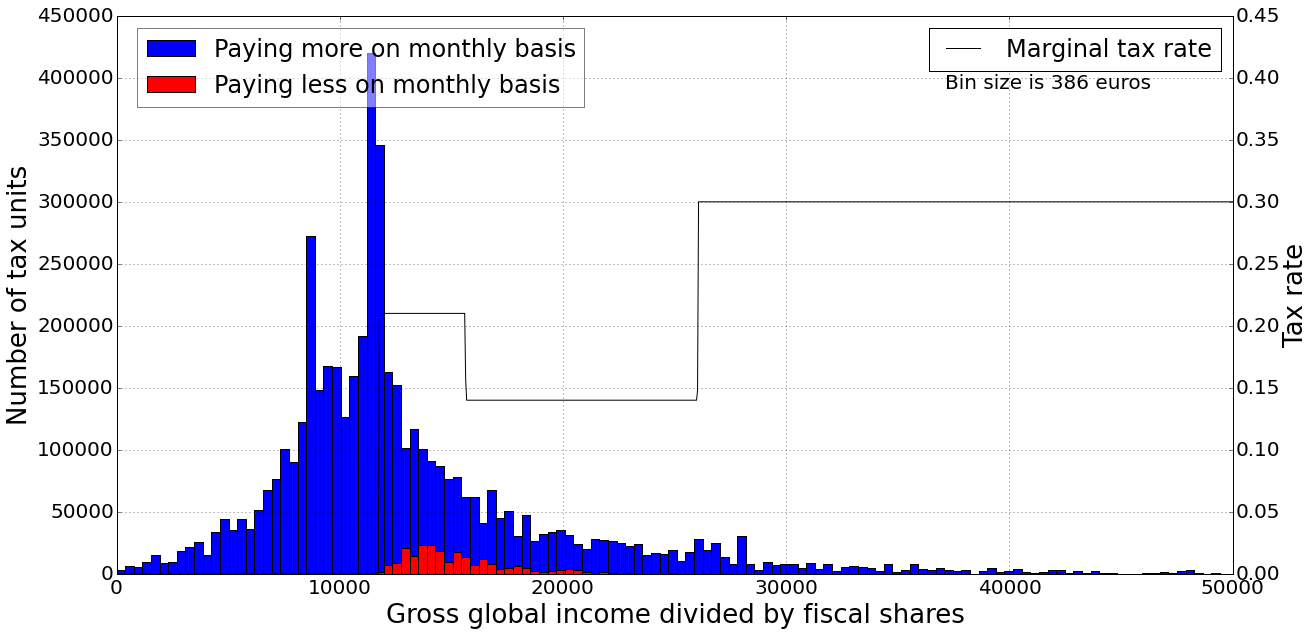
\includegraphics[ width=\textwidth]{monetary_winner_looser.png}
\end{center}
\end{figure}


\autoref{fig:monetary_winner_loosers} shows the number\ of monetary winners
and losers among fiscal households according to their normalized tax
base.\footnote{In order to make them comparable we divided the taxable income
by the number of fiscal shares (such that they are normalized to face the same
tax schedule).}\hfill when we implement the monthly tax system instead the equal
payment system. We see that losers (in blue -- or light grey) represent the
vast majority (more than 95\%) with respect to winners (in red-- or black). As
expected, we see that the taxpayers that pay less on a monthly basis are the
one located around the concave part of the tax scheme: those whose some
monthly income belongs to the 22.5\% tax bracket. There are also winners
because of the threshold exemption which also introduces a small non-convexity.\ 

\paragraph{Welfare Analysis.}

To estimate the welfare gains and losses, we need to estimate a utility
function.\ The theory of equal sacrifice provides a sound theoeretical basis
to estimate such a utility function. Young (\cite{young1990progressive})
provides a method to test the theory of equal sacrifice against data.\ It
shows that the fit is not that bad on various examples, including the US
income tax.\ We did it on French data and we used the estimated utility
function to calibrate the welfare changes.\ 

The yearly disposable income $z$ is obviously computed as
\[
Z=\sum_{1}^{12}z_{t}=\sum_{1}^{T}y_{t}-g_{t}(y_{t})
\]


The best fit for an utility function defined on yearly basis we obtain is%

\[
U(Z)=-\left(  Z\right)  ^{-0.89}.
\]


We define the utility function to a monthly basis as%

\begin{equation}
u_{t}(z_{t})=\frac{-\left(  12{z_{t}}\right)  ^{-0.89}}{12}%
\end{equation}


in order the sum over the year gives the yearly utility $U$.

\begin{figure}[ptb]
\caption{The distribution of utility gains and losses for the monthly and monthly compensated schemes vs equal split }%
\label{fig:sutility_1}
%article_graphs_simulation_results-new_monthly [91] 1/06/2017
\par
\begin{center}
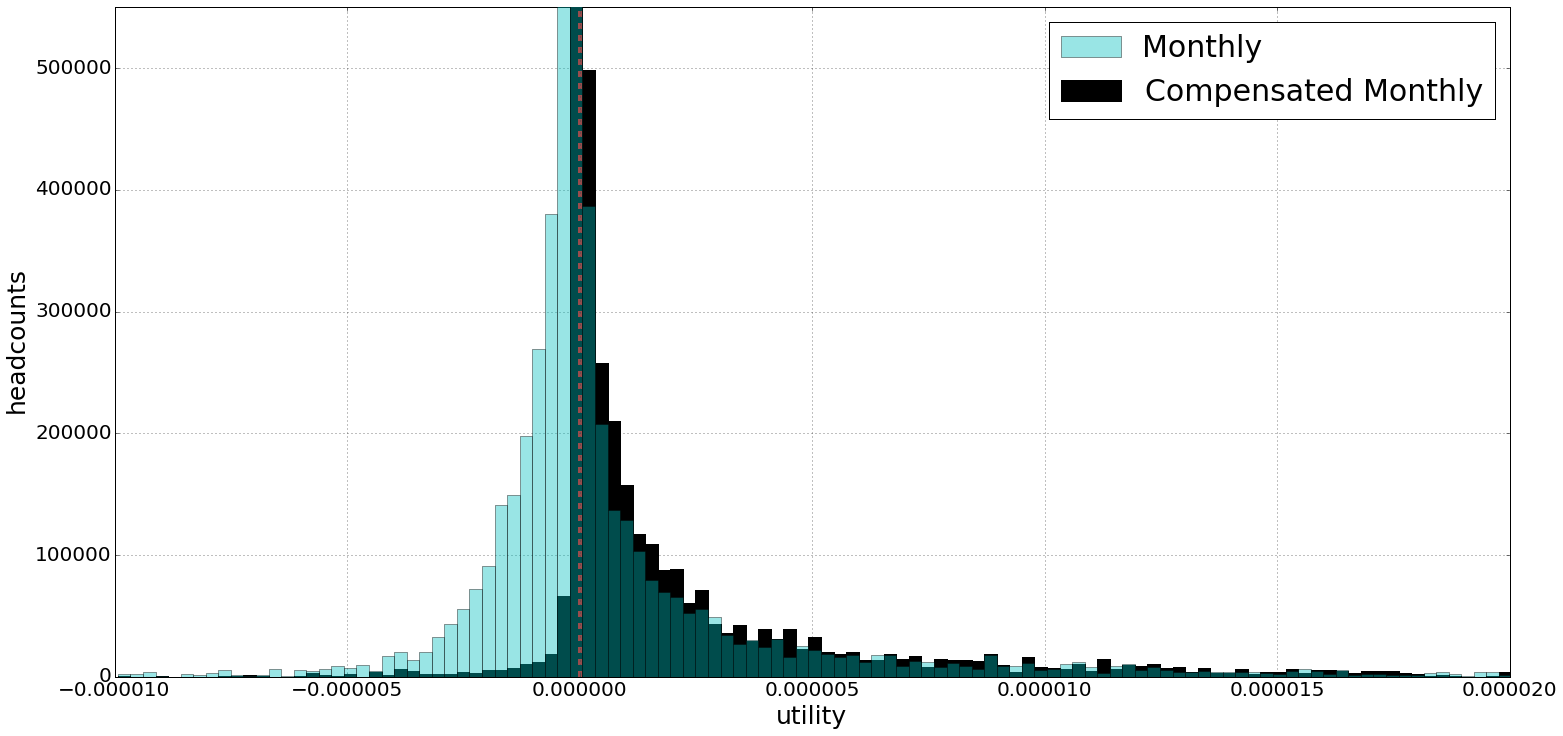
\includegraphics[ width=\textwidth]{utility_1.png}
\end{center}
\end{figure}
%\begin{figure}[H]
%\begin{center}
%\caption{ }
%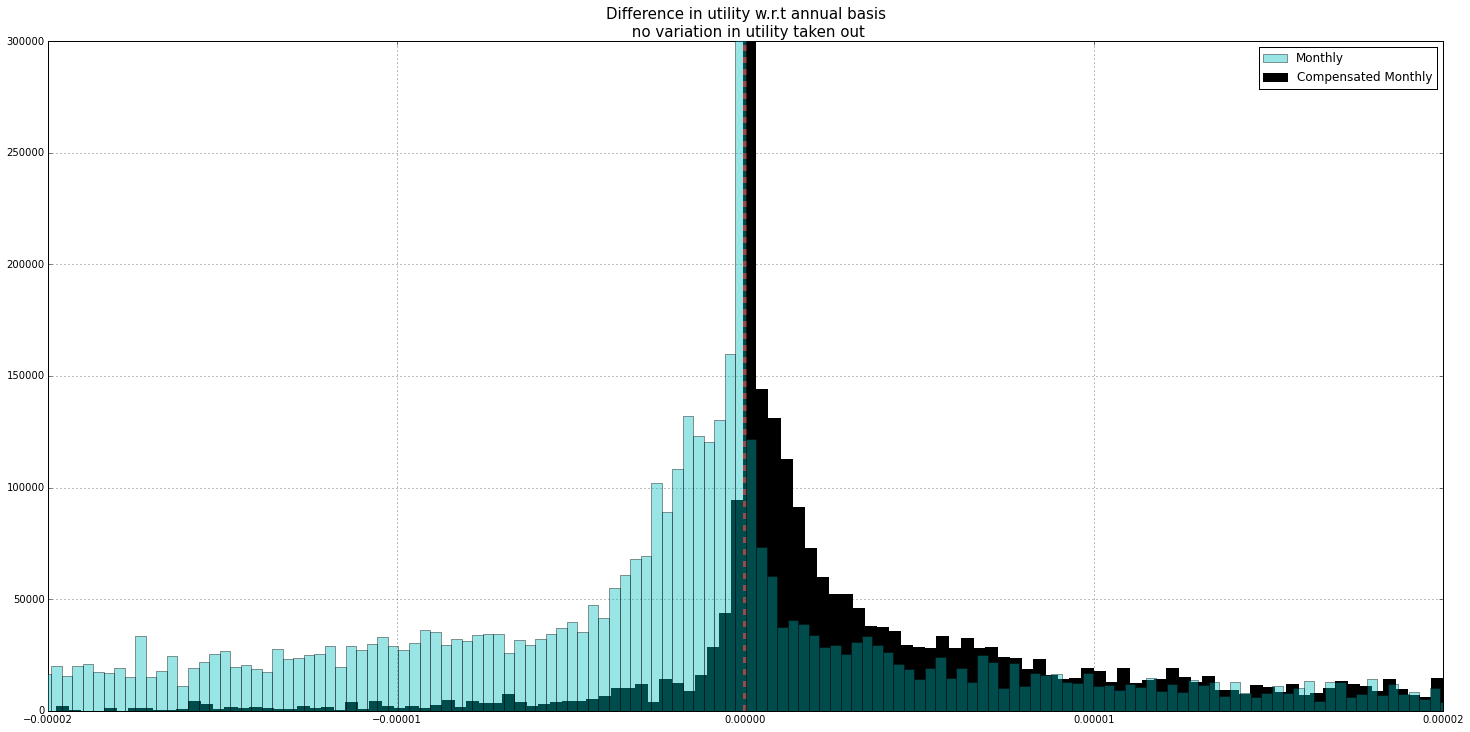
\includegraphics[ width=\textwidth]{utility_2.png}
%\label{fig:sutility_2}
%\end{center}
%\end{figure}


\autoref{fig:sutility_1} shows all losers and winners by utility points bins
gains or loss. Utility gains with the monthly tax scheme are in cyan and dark
green while the utility gains with the compensated monthly tax scheme are in
black and dark green.

%\autoref{fig:sutility_2} take out outliers (less than 0.00002 utility points of variation, 25 \% of the sample) and null utility variation taxunit.


We see as expected that there are losers (10\% of the sample) and winners
(7.4\%) with the monthly tax scheme. The former concerns taxpayers that have
higher amount of tax to pay and benefit less from income smoothing over the
year. With the monthly compensated tax scheme, almost people are net gainers
from the reform. For the few losers (2\%), there are two reasons which approximatively are equally important. For 50\%
of them, their income falls down on the concave part of the tax scheme, and
for 50\% of them because of the collection threshold of the tax.

\paragraph{Comparison with Vickrey tax scheme}

We have implemented Vickrey tax scheme as defined in \autoref{eq:vickrey} with
the reference period being year 2009 and the sub-period span being the month.
In \autoref{fig:vickrey_gain} we can see the difference in utility of the
monthly compensated tax scheme and the Vickrey tax scheme viz the equal
payment scheme. The grey colour shows the overlap between the two histograms;
the black is specific to Vickrey and the cyan to the monthly compensated.\ 

\begin{figure}
\caption{ The distribution of utility gains and losses for the Vickrey and monthly compensated schemes vs equal split}%
\label{fig:vickrey_gain}
%article_graphs_simulation_results-new_monthly [] 2/06/2017
\par
\begin{center}
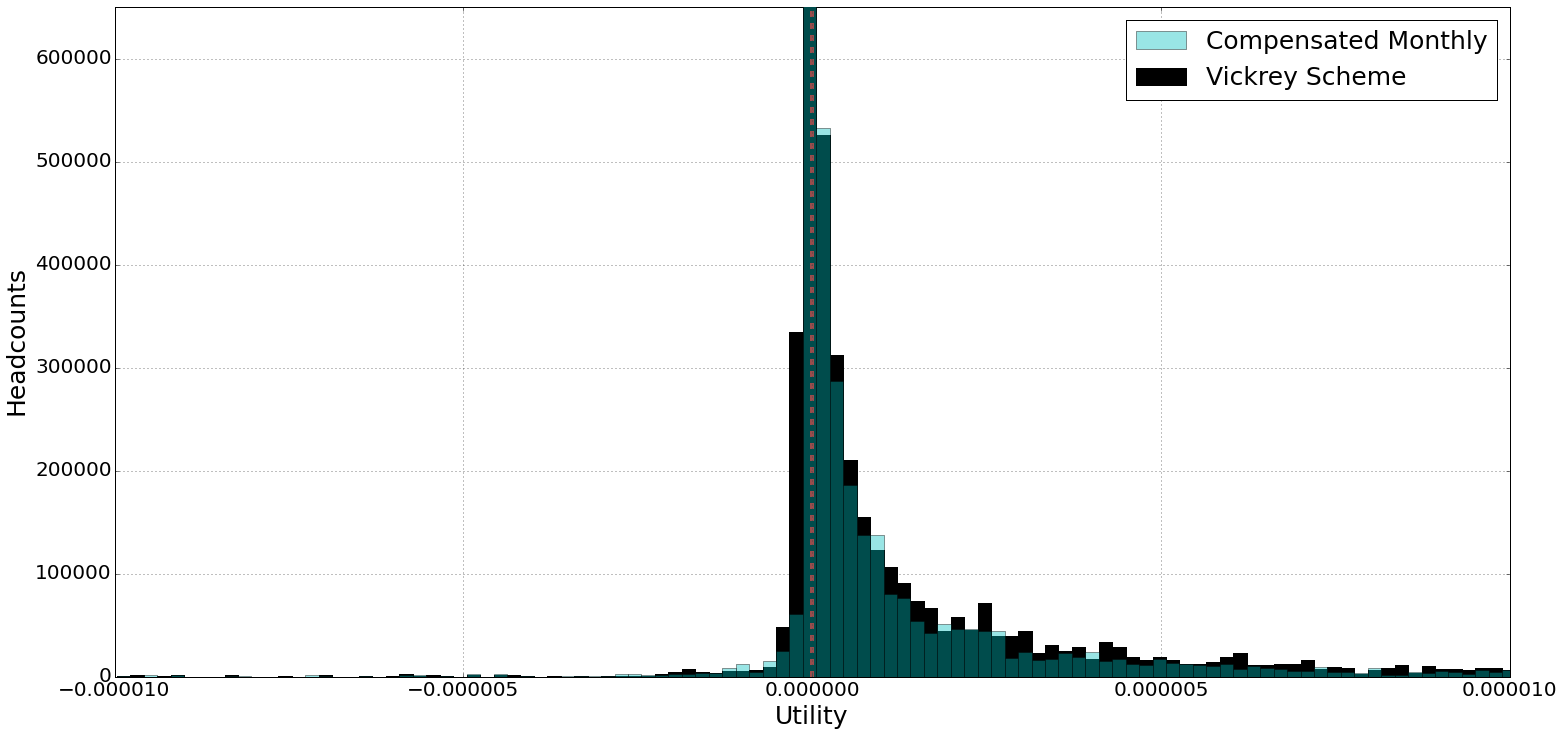
\includegraphics[ width=\textwidth]{vickrey_utility.png}
\end{center}
\end{figure}

The first message is that the two distributions are quite close and both
mechanisms have similar impacts in terms of providing a smoothing
income.\ Both mechanisms make the individuals happier compared to the equal
payment scheme but the proportion of winners is higher with Vickrey than with
Monthly compensated (13,4\% againts 9,2\%). In addition on average Vickrey
compensation scheme leads to higher utility gains than the monthly compensated
tax scheme.\ However, a higher fraction of the population has a loss in
utility with the Vickrey tax scheme (6.2\%) compared to equal payment than
with the monthly compensated one (2\%). These people are taxpayers that earn
less at the beginning of the year than at the end. It is an echo of the
results found in the theoretical section.

\autoref{Utility with schemes} computes the average utility for the different tax systems.
Average utility $U$ is of $-1253\ast10^{-7}$, $-1250\ast10^{-7}$,
$-1249\ast10^{-7}$, $-12444\ast10^{-7}$, for respectively the annual basis
tax, the monthly tax, the monthly basis compensated tax, and the Vickrey
scheme. Mean utilitarian gains of an increase in frequency is of $3\ast
10^{-7}$, and gain from an increase with compensation is of $4\ast10^{-7}$,
while the Vickrey scheme entails a gain of $9\ast10^{-7}$ utility points.

\begin{table}[ptb]
\caption{Utility with the different tax schemes}
\label{Utility with schemes}
%descrptive_statistics-new_monthly_2 12/06/2017 [31]
\centering
\resizebox{\textwidth}{!}{\begin{tabular}{lcccccccc}
& \multicolumn{4}{c}{Without equivalent scale} & \multicolumn{4}{c}{With equivalent scale} \\
\cmidrule(lr){2-5}\cmidrule(lr){6-9} \morecmidrules
\cmidrule(lr){2-5}\cmidrule(lr){6-9}
Tax scheme  & Equal split & Monthly & Compensated & Vickrey&Equal split& Monthly & Compensated & Vickrey\\
\midrule
Aggregate &-4206.78&-4195.98&-4194.63&-4178.36&-7599.73&-7582.93&-7579.59&-7552.6   \\
Average &-1.2529 $ \times 10^{-4}$ &-1.2497 $ \times 10^{-4}$ &-1.2493 $ \times 10^{-4}$ &-1.2444 $ \times 10^{-4}$ &-2.2634 $ \times 10^{-4}$ &-2.2584 $ \times 10^{-4}$ &-2.2574 $ \times 10^{-4}$ &-2.2494$\times 10^{-4}$ \\
\bottomrule
\end{tabular}}\end{table}

In order to take into account the effect of joint taxation, we also implement
the OECD equivalent scale to compute utility. The ranking of tax systems is similar.\ 

So the message that comes out of this simulation is the following.\ The
monthly compensated mechanism is more inclusive (less losers) but the gains
are more modest than with Vickrey.\ We conclude this empirical section as well
as the theoretical section that this is a closed contest between Vickrey and
Monthly compensated payment system. It is too close to call.\ \medskip

\section{Conclusion}

In this article the within-year frequency of the tax and the tax basis for a
monthly payment were under scutiny. We have proven given some standard
hypothesis that it can be Pareto-improving to adopt a monthly tax base for the
monthly payment. We have then tried to confront our theoretical framework to
reality by implementing our prescriptive reform to the French income tax.

We have shown that there is a mismatch between our framework where the income
tax convex and reality in developed countries such as US, UK\ and France:
taxes on income are not convex and it has some adverse implication in terms of
disposable income in a dynamic setting: convex tax schemes promote steady
incomes and tax more heavily varying income, while concave tax schemes
subsidize varying income. The dataset we used shows that most varying incomes
are located at the bottom of the distribution, where precisely the income
tax-benefit system is not convex.

We have then run the microsimulation model \emph{OpenFisca} to estimate the
impact of a switch from a between-month equal split system to monthly
compensated based system.\ We have quantified monetary gains and loss for
taxpayers and identified losers and winners. We have then performed a welfare
analysis based on the equal sacrifice principle to determine losers and
winners in terms of utility of the switch.

The main results is that in average the Vickrey performs better.\ The embodied
insurance mechanisme works better whatever the convexity of the tax scheme,
whereas that of the Monthly compensated supposes the convexity of the tax
scheme.\ In a true sense, this latter mechanism is penalized by the lack of
convexity in the bottom part of the income distribution.\ However, a weakness
of the Vickrey systeme has been revealed both by the theory and by the
data.\ It works less well for increasing income stream within a year.\ This
configuration is unfortunately that for which the lack of precautionary saving
is the most detrimental.\ 

Those results are driven by within-year income variability. Most income
variability studies in developed countries look at year to year incomes, to
the notable exception of \citet{Hills2006} who looks at week-by-week effective
disposable incomes of 93 poor families over a year in the UK. \footnote{We can
also note \citet{jenkins2000current} who studied the difference between
snapshot of current income vs. synthesize annual income on the observation of
the distribution of income, their findings is that it has nearly no impact.}
\citet{Hills2006} emphasize that over nine tenth of those families has monthly
income that vary over 10\% of their average income
\footnote{\quote{Only seven of the 93 families had incomes fitting our
"highly stable" pattern, that is, varying less than 10 per cent either way
from their annual average. Only a third had income in at least eleven
periods within 15 per cent of their mean, and within 25 per cent of it in
any other periods.}} and half of the families in the sample has nothing left
over for savings, and a quarter for which outgoings exceeded income.
Literature on saving behavior --always yearly based-- underline that bottom of
the distribution has very high marginal propensity to consume.
\footnote{Carrolls, etc, choisir les bonnes r\'{e}f\'{e}rences.} Those facts
suggest that a large parts of the bottom of the distribution cope with
whatever is their monthly disposable income and gives credit to our
"no-saving" framework. Poor savings and income variability can have huge
impact on citizen well being, this suggest that the tax-benefit scheme should
be studied in a non purely static models with those effects in mind.

Similarly to \citet{brewer2010means} \footnote{" The assessment period and
timing of taxes and transfers In most countries, individual income taxes are
assessed on annual income, and transfers often assessed on a monthly basis (in
the UK, weekly). Standard economic models predict that families should budget
over long time periods, by borrowing (or using credit) and saving. If families
have fluctuating incomes but are able to smooth consumption over time by
borrowing and saving, then income assessed over a longer period of time is a
better measure of economic welfare or well-being than income assessed over a
short period of time. In reality, costs of using financial services and other
credit market failures, low levels of literacy, numeracy and financial
education, and self-control problems with savings all create significant
departures from the standard model. These departures are likely to be more
prevalent amongst low-income families, and tend to lead to such families
budgeting consumption over short periods of time, such as a month or a
fortnight. It therefore seems desirable to operate transfers for low-income
families on a \textbf{high-frequency basis}, and operate taxes on higher
incomes on a lower frequency, such as annual."}, our public prescription is
that bottom of the distribution, tax-benefits should be based on
high-frequency in order to smooth disposable income. As we have shown, this is
compatible with not increasing the size of transfer payments to the bottom
part of the distribution.

Increasing tax frequency could allow for a decrease of the size of the refund
which can have some macroeconomic consequences. Such situation has been
empirically studied by
\citet{shapiro1993consumer,shapiro2003consumer,shapiro2009did} that study the
impact on aggregate demand of the US tax-refund.

Those issues open avenues for further research that should be investigated.
Optimal taxation is for most contributions developed in a static framework.
Studying the incentives and its impact on the optimal tax scheme in a dynamic
setting might lead to different public policy prescriptions as the one
prescribed by actual models.

\newpage

\addcontentsline{toc}{section}{References}
\bibliography{tax_frequency}

%%%%%%%%%%%%%%%%%%%%%%%%%%%%%%%%%%%%%%%%%%%%%%%%%%%%%%%%%%%%%%%%%%%%%%%%%%%%%%%%%%%%%%%%%%%%%%%%%%%%%%%%%%%%%%


\ifx\isEmbedded\undefined
\newpage
%\bibliography{tax_frequency}
\end{document}
\else \fi